%%%%%%%%%%%%%%%%%%%%%%%%%%%%%%%%%%%%%%%%%%%%%%%%%%%%%%%%%%%%%%%%%%%%%%%%%%%%%%%%%%%%%%%%%%%%%%%%%%%
% Chapter 2 -> Background
% Author: Eduardo G Gusmao
%%%%%%%%%%%%%%%%%%%%%%%%%%%%%%%%%%%%%%%%%%%%%%%%%%%%%%%%%%%%%%%%%%%%%%%%%%%%%%%%%%%%%%%%%%%%%%%%%%%
\chapter{Background}
\label{cha:background}

\graphicspath{{chapter2/figs/}}

% This chapter
In this chapter we provide the background information required for the understanding of this thesis. First, we introduce the necessary biological concepts (Section~\ref{sec:gene.regulation}). Next, we present the biological experimental techniques which are the main sources of data used in our analysis (Section~\ref{sec:ngs.methods}). Then, we introduce the problem which we are going to address in this thesis -- the computational identification of active transcription factor binding sites (Section~\ref{sec:active.binding.site.detection}). Subsequently, we discuss the state-of-the-art computational solutions used to process modern biological experimental data and address the aforementioned problem (Section~\ref{sec:computational.footprinting.methods}). Finally, we close this chapter with concluding remarks on the definitions made in this chapter and a brief motivation on our strategy to tackle the problem of identification of active transcription factor binding sites (Section~\ref{sec:discussion.2}).

%%%%%%%%%%%%%%%%%%%%%%%%%%%%%%%%%%%%%%%%%%%%%%%%%%%%%%%%%%%%%%%%%%%%%
% Section: Gene Regulation
%%%%%%%%%%%%%%%%%%%%%%%%%%%%%%%%%%%%%%%%%%%%%%%%%%%%%%%%%%%%%%%%%%%%%
\section{Gene Regulation}
\label{sec:gene.regulation}

% Introduction & this section
In this thesis we will focus on the biological field of gene regulation. Such research area focuses on the understanding of the cellular mechanisms behind the temporal and spatial expression of different genes on different cellular conditions. We start this section by describing the basic concepts of molecular biology (Section~\ref{sec:basic.concepts.molecular.biology}). Then, we describe the main biological processes regarding gene regulation (Section~\ref{sec:eukaryotic.regulation}). Finally, we discuss the role of chromatin dynamics on such regulatory processes (Section~\ref{sec:chromatin.dynamics}).

%%%%%%%%%%%%%%%%%%%%%%%%%%%%%%%%%%%%%%%%%%%%%%%%%%%%%%%%%%%%%%%%%%%%%
% Section: Basic Concepts of Molecular Biology
%%%%%%%%%%%%%%%%%%%%%%%%%%%%%%%%%%%%%%%%%%%%%%%%%%%%%%%%%%%%%%%%%%%%%
\subsection{Basic Concepts of Molecular Biology}
\label{sec:basic.concepts.molecular.biology}

% Introduction
In this thesis we focus on two important macromolecules which are found inside cells: proteins (composed by amino acids) and nucleic acids (composed of nucleotides). The proteins assume many roles: catalysis of chemical reactions (enzymes), metabolite processing, cell signaling, regulation of the production of more proteins, structural function and others. Given such great variety of processes in which proteins are associated with, one might regard these macromolecules as having a central role in the maintenance of living organisms. The nucleic acids can be of two types: the deoxyribonucleic acid (DNA) and ribonucleic acid (RNA). The main function of the DNA is to store the hereditary information of the organism. It is based on such information that new proteins are generated by cellular processes. The RNA have many important functions; however we will not focus on this molecule in this work.

% DNA structure
The DNA molecule is formed by a double helix of paired nucleotide chains, each of which composed of the nucleotide types: adenine (A), cytosine (C), guanine (G) and thymine (T). Each nucleotide is composed by a sugar (deoxyribose), a phosphate group and a nitrogenous base (which determines the nucleotide type). Within each DNA strand of the double helix, nucleotides are connected through phosphodiester bonds (strong covalent bonds). Between each DNA strand, nucleotides are paired and connected through hydrogen bonds (weaker than covalent bonds). Cytosines always pair with guanines and adenines always pair with thymines. Because nucleotides are paired between the double helix structure, is very common to refer to nucleotides as base pairs (bp). The Figure~\ref{fig:alberts_dna_structure} depicts a graphical representation of the DNA molecule.

% Figure - DNA structure
\begin{figure}[h!]
\centering
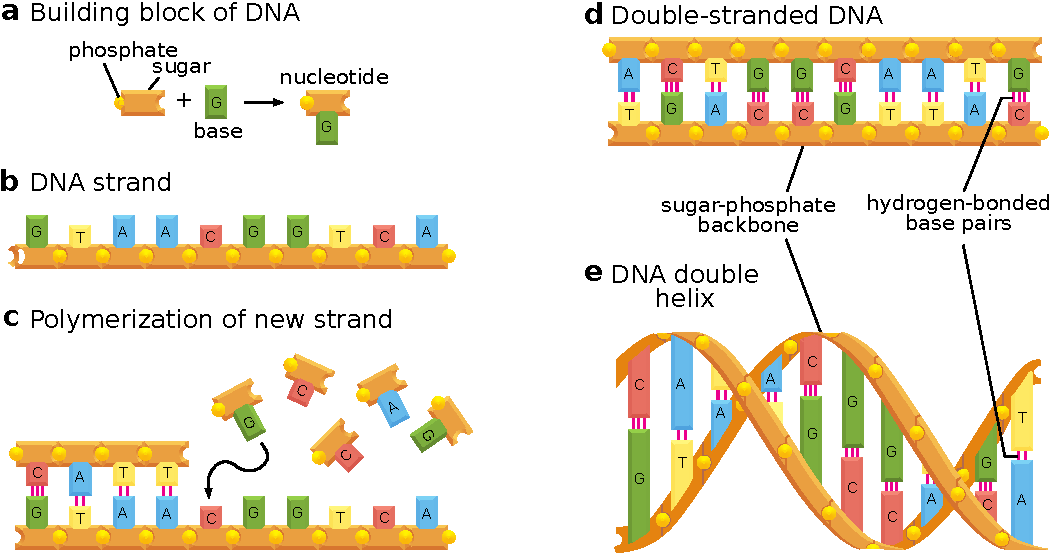
\includegraphics[width=0.99\textwidth]{alberts_37_dna_structure}
\caption[DNA structure]{\textbf{DNA structure.} (\textbf{a}) Representation of the DNA's building block -- the nucleotide. (\textbf{b}) Multiple nucleotides from all possible types (A, C, G and T) form a single strand of DNA, which in humans can be as long as \approxy$250,000,000$ nucleotides. (\textbf{c}) The DNA generally occurs as a double strand. The biological process of polymerization allows the addition of nucleotides to a single strand, forming the DNA double strand. Cytosines (C) always pair with guanines (G) connected through three hydrogen bonds (pink lines); and adenines (A) always pair with thymines (T) through two hydrogen bonds. (\textbf{d}) Linear scheme of the double DNA strands. (\textbf{e}) Double helix structure of the double-stranded DNA molecule. This is the general structure in which the DNA occurs in nature. \emph{Source: Alberts et al.}\cite{alberts2007} (modified to fit thesis format and/or clarify key points).}
\label{fig:alberts_dna_structure}
\end{figure}

% Protein structure dictates function
Proteins are chemical compounds with high molecular weight formed by a variable-length chain of amino acids. The amino acids that forms the proteins are composed of a central carbon atom which binds to a hydrogen, a carboxyl group, an amine group and a side chain. The side chain may be of various types and dictates the type of the amino acid. There are 20 amino acid types which are more common to be found at proteins. The specific order of each amino acid type in a protein determines its three-dimensional structure. It is well-known that the protein's function is directly related to its structure. The simple substitution of one amino acid in the proteic chain is sufficient to modify the protein three-dimensional conformation leading to a reduced functional capability or complete protein dysfunction. The Figure~\ref{fig:villarreal_protein} shows the different levels of protein structural conformation.

% Figure - Protein structure
\begin{figure}[h!]
\centering
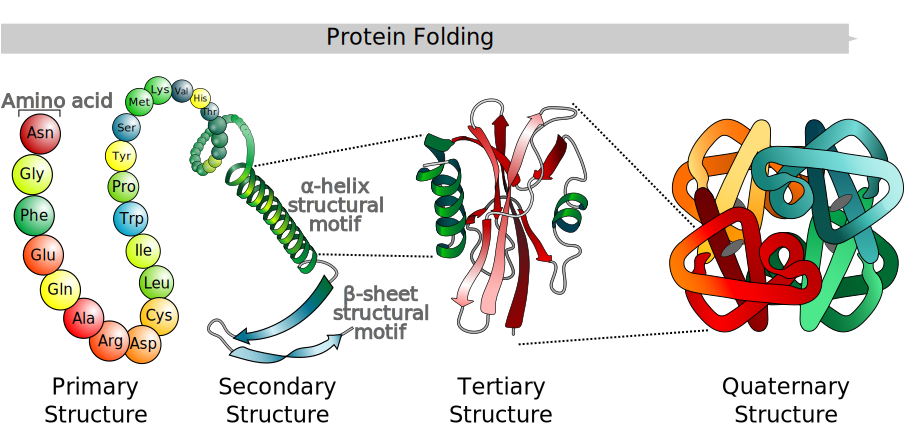
\includegraphics[width=0.95\textwidth]{villarreal_protein}
\caption[Protein structure]{\textbf{Protein structure.} Proteins are formed by building blocks termed amino acids. The chain of amino acids that forms a specific protein is the protein's primary structure. The protein secondary structures, such as $\alpha$-helixes or $\beta$-sheets, are formed through the natural folding of the amino acid chain given their physicochemical properties. The terciary structure are composed by a number of secondary structures forming a stable protein unit. Finally, the quaternary structure represents the aggregation of multiple protein units to form fully functional protein. \emph{Source: Mariana R. Villarreal} (modified to fit thesis format and/or clarify key points).}
\label{fig:villarreal_protein}
\end{figure}

% Central dogma introduction
The process in which proteins are created based on the information encoded in the cell's DNA is called the ``central dogma of molecular biology''. Here, the key parts of this process, which aid in the understanding of this work, are presented. These key parts are: (1) the initiation, (2) the transcription and (3) the translation.

% Central dogma
During the initiation phase, a number of proteins called transcription factors bind in the DNA and recruit another protein called RNA polymerase (Figure~\ref{fig:lodish_central_dogma}a). The DNA region in which these transcription factors and RNA polymerase bind to start transcription is called promoter. Then, in the transcription phase, the RNA polymerase scans the DNA and creates an RNA molecule, based on the information encoded in the DNA (Figure~\ref{fig:lodish_central_dogma}b). The part of the DNA which is transcribed by the RNA polymerase is called gene. Finally, in the translation phase, the newly-generated RNA migrates outside the cell's nucleus and a protein called ribosome scans the RNA and creates a protein molecule based on the information encoded in the RNA (Figure~\ref{fig:lodish_central_dogma}c). The rate in which the transcription occurs for a particular gene is called the gene's expression.

% Transcription - strands and order
It is important to mention that, although only one of the DNA strands is read during the transcription process, both strands contain information necessary to produce RNA. Another important issue is the orientation of these two DNA strands. Each strand has two extremities: one corresponding to a hydroxyl group attached to the $3^\prime$ carbon atom of the sugar; and the other corresponding to the phosphate group attached to the $5^\prime$ carbon atom of the sugar. For this reason, processes involving the sliding of proteins in DNA have two orientations: forward ($5^\prime \rightarrow 3^\prime$) and reverse ($3^\prime \rightarrow 5^\prime$). The different strands in the DNA helix are attached to each other in opposite (anti-parallel) orientations. The transcription always occurs in the forward orientation.

% Figure - Central dogma of molecular biology
\begin{figure}[h!]
\centering
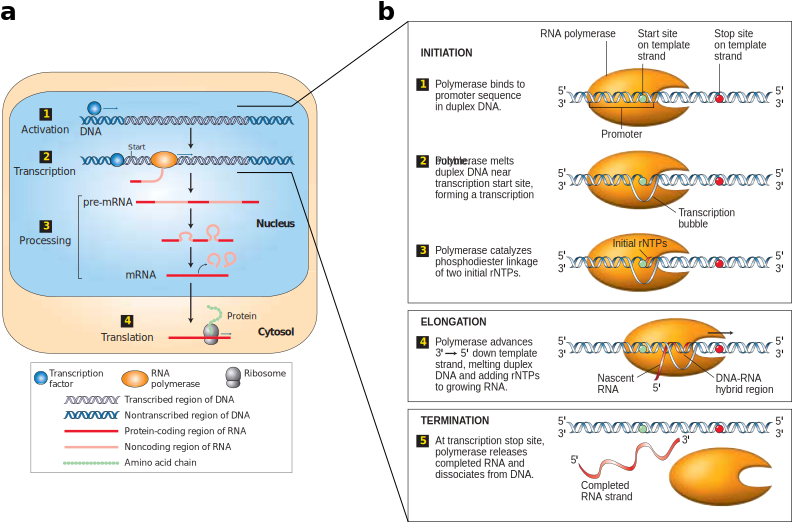
\includegraphics[width=0.9\textwidth]{lodish_30_central_dogma}
\caption[Central dogma of molecular biology]{\textbf{Central dogma of molecular biology.} Depiction of the main steps of the central dogma of molecular biology necessary to create a protein molecule from the information encoded within the DNA molecule. Here we show the steps: (\textbf{a}) initiation, (\textbf{b}) transcription and (\textbf{c}) translation. \emph{Source: Lodish et al.}\cite{lodish2007} (modified to fit thesis format and/or clarify key points).}
\label{fig:lodish_central_dogma}
\end{figure}

%%%%%%%%%%%%%%%%%%%%%%%%%%%%%%%%%%%%%%%%%%%%%%%%%%%%%%%%%%%%%%%%%%%%%
% Section: Eukaryotic Regulation
%%%%%%%%%%%%%%%%%%%%%%%%%%%%%%%%%%%%%%%%%%%%%%%%%%%%%%%%%%%%%%%%%%%%%
\subsection{Eukaryotic Regulation}
\label{sec:eukaryotic.regulation}

% Introduction - eukaryotes
Living organisms can be divided into two groups: (1) prokaryotes -- the organism's genetic material (i.e. the DNA) is located in the cell's cytoplasm and presents a circular structure and (2) eukaryotes -- the organism's cells have a nucleus which contains, among other structures, the DNA. Here, we will focus on eukaryotes. Most eukaryotes have more than one DNA molecule, which are termed chromosomes. The set of a cell's chromosomes is called genome. Furthermore, some organisms present more than one copy of a chromosome. The human genome presents two copies of $22$ different chromosomes (referred to based on a number between 1--22) and two additional chromosomes (termed X and Y), which determines the individual's biological gender. This adds up to a total of $46$ chromosomes and classify humans as diploid organisms (have two copies of each chromosome).

% Introduction - Trascriptional regulation
The transcription initiation was previously described as the step in which the RNA polymerase binds to the promoter region in order to start the process of transcription. Nevertheless, there are many factors that contribute to the expression of particular genes in particular types/stages/conditions of a cell. We call ``gene regulation'' the wide range of mechanisms that are used by cells to increase or decrease the production of specific gene products. Gene regulation may happen in different stages of the central dogma. However, most part of the regulatory events happens at the transcription initiation level. A major role of the regulation at this level is played by proteins termed transcription factors, which use their physicochemical properties to direct the intensity level in which gene products are created. The transcription factors bind to DNA regions called transcription factor binding sites which can be close (promoter region; $< $\approxy$1,000$ bp from the transcription start site) or far (distal regulatory regions; up to \approxy$1,000,000$ bp) from the gene. Different transcription factors may bind to different transcription factor binding sites to increase or decrease the expression of genes. The Figure~\ref{fig:gusmao_gene_regulation} shows a graphical representation of a basic regulatory landscape of a gene. The number of regulatory elements vary between genes; however the construct of transcription factor and their DNA binding sites are generally present.

% Figure - Regulatory elements
\begin{figure}[h!]
\centering
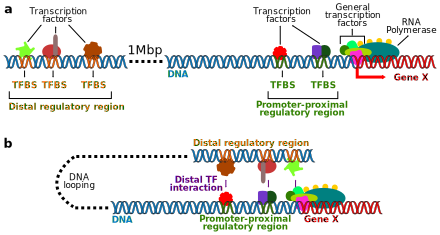
\includegraphics[width=0.80\textwidth]{gusmao_gene_regulation}
\caption[Basic regulatory landscape of a gene]{\textbf{Basic regulatory landscape of a gene.} (\textbf{a}) Schematic representation of a typical gene regulatory region with proximal and distal regulatory regions, composed of transcription factor binding sites (transcription factor binding sites), which are regions in the DNA being bound by proteins called transcription factors (transcription factors). The promoter typically spans less than $1$ Kbp and is composed of: (1) a core promoter -- where the transcriptional machinery is being bound and (2) promoter-proximal regulatory region -- where transcription factors bind to increase/decrease gene expression. The distal regulatory regions can be located up to $1$ Mbp from the promoter. Among others, they can be categorized as: (1) enhancers -- where transcription factors bind to increase gene expression and (2) silencers -- usually decreasing or completely silencing expression. (\textbf{b}) These distal elements may contact the core promoter or proximal promoter through a mechanism that involves looping out the intervening DNA.}
\label{fig:gusmao_gene_regulation}
\end{figure}

% Protein motifs
The transcription factors contain a specific part (formally called ``domains'') within their structure, termed active site, which enables them to bind to the DNA. There is a relatively short number of smaller structural variants (which compose the final protein structure) in comparison to the number of different protein types. Some of these structural variants, including the ones containing active sites, are repeated between different protein. These DNA-binding protein domains usually have affinities towards specific DNA sequences. These affinity sequences are termed ``DNA motifs''. The Figure~\ref{fig:gusmao_binding_type} shows four DNA-binding protein domains and examples of proteins that contain such domains and their respective DNA binding affinity motifs.

% Figure - Different protein-DNA binding types
\begin{figure}[h!]
\centering
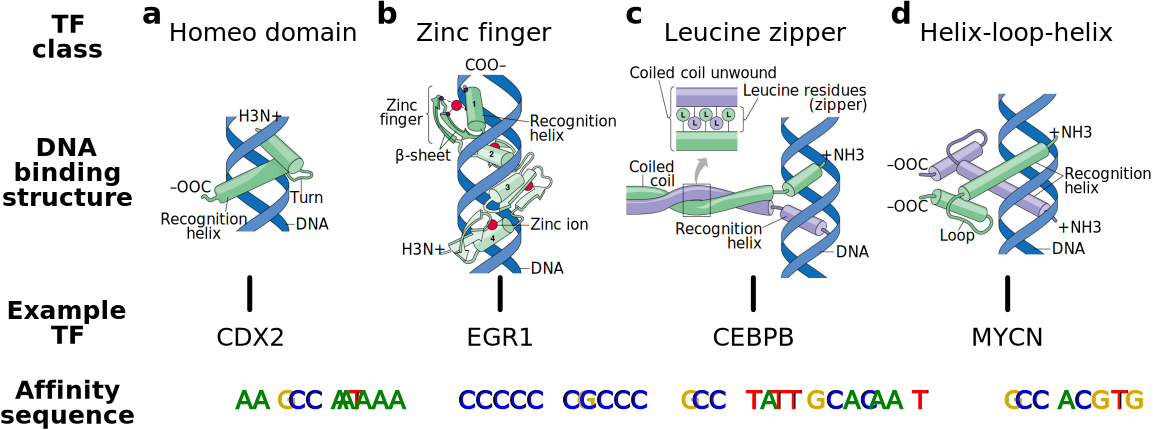
\includegraphics[width=0.99\textwidth]{gusmao_binding_type}
\caption[Different protein-DNA binding types]{\textbf{Different protein-DNA binding types.} We show graphical representations of different protein-DNA binding types (top) and examples of proteins with such binding domain type and their DNA sequence binding affinity information (bottom). We show four DNA-binding transcription factor classes: (\textbf{a}) Homeo domain (also known as helix-turn-helix), (\textbf{b}) zinc finger, (\textbf{c}) leucine zipper and (\textbf{d}) helix-loop-helix. This motivates the idea that, although there are many DNA-binding proteins, they usually have a few DNA-binding domains.}
\label{fig:gusmao_binding_type}
\end{figure}

%%%%%%%%%%%%%%%%%%%%%%%%%%%%%%%%%%%%%%%%%%%%%%%%%%%%%%%%%%%%%%%%%%%%%
% Section: Chromatin Dynamics
%%%%%%%%%%%%%%%%%%%%%%%%%%%%%%%%%%%%%%%%%%%%%%%%%%%%%%%%%%%%%%%%%%%%%
\subsection{Chromatin Dynamics}
\label{sec:chromatin.dynamics}

% Chromatin structure 1
The DNA is not isolated in the cell nucleus. Instead, it is found wrapped in proteic complexes which is associated to the compaction of the DNA within the cell nucleus and many regulatory events. Such DNA$+$protein structure is termed chromatin. The DNA is found wrapped in a set of eight proteins called histone complex, which are generally composed of four pairs of histones named H2A, H2B, H3 and H4. The unit composed by the DNA wrapped in approximately $1.65$ turns (\approxy$147$ bp) around the histone complex is called nucleosome. From this lower level structure (nucleosome) the chromatin structure can be compacted in many levels. This compaction organization is depicted in Figure~\ref{fig:lodish_chromatin_structure}. Briefly, the chromatin can be found in a very condensed structure which does not allow transcription initiation (termed heterochromatin, or simply ``closed chromatin''); or in a decondensed form, allowing transcription initiation and gene expression (termed euchromatin, or simply ``open chromatin'').

% Figure - Chromatin conformation
\begin{figure}[h!]
\centering

\includegraphics[width=0.85\textwidth]{lodish_420_chromatin_structure}
\caption[Chromatin conformation]{\textbf{Chromatin conformation.} The nuclear DNA have many compaction levels. (\textbf{a}) The lowest chromatin level corresponds to the DNA double helix. (\textbf{b}) The DNA double helix loops around the hisone complexes forming the nucleosomes. (\textbf{c}) With additional structural proteins, the nucleosomes are packed in a structure termed $30$-nm fiber. (\textbf{d}) The $30$-nm fiber is further compacted in many compaction levels with the aid of further structural proteins. (\textbf{e}) The higher degree of chromatin compaction is represented as the chromosome in the cell's metaphase.  \emph{Source: Lodish et al.}\cite{lodish2007} (modified to fit thesis format and/or clarify key points).}
\label{fig:lodish_chromatin_structure}
\end{figure}

% Chromatin structure 2
Different parts of the genome can be open and closed at different times, allowing a specific set of genes to be expressed under different cell conditions. This is one of the main mechanisms in which we are able to observe such a high number of different cells, each of which expressing a different set of genes, given that they all share the same underlying genomic information encoded in the DNA. The chromatin can switch between closed and open states via two major chromatin remodeling mechanisms: (1) covalent post-translational histone modifications by specific enzymes such as histone acetyltransferases (HATs), deacetylases, methyltransferases and kinases and (2) ATP-dependent chromatin remodeling complexes which either move, eject or restructure nucleosomes. Here, focus on the post-translational histone modifications.

% Histone modifications
The histone proteins' n-terminal usually protrudes from the nucleosome and is termed histone tail. Histone tails can undergo post-translational chemical modifications at specific amino acids. Such modifications include the methylation (addition of a methyl group), acetylation (addition of an acetyl group), phosphorylation (addition of a phosphoryl group), ubiquitylation (addition of a ubiquitin protein) and sumoylation (addition of SUMOs -- small ubiquitin-like modifiers). These modifications have a specific nomenclature dictated by: histone type, amino acid type, amino acid position within the histone tail and modification type. For instance, ``H3K4me1'' refers to the monomethylation (me1) of the fourth lysine (K4) of the tail of histone H3.

% Histone modification effects on chromatin
The histone modifications are directly associated to regulatory events since they change the accessibility of proteins to the DNA in the chromatin, enabling or disabling the binding of transcription factors. For instance, the HATs are able to transfer an acetyl group to certain amino groups of histone tail's lysine side chains. In doing so, they neutralize the lysine's positive charge and makes the interactions between histones and DNA weaker. Consequently, the DNA is more accessible for transcription factor binding. The Figure~\ref{fig:lall_histone_modifications} displays the known effects of modifications in lysines in the tail of histone H3.

% Figure - Main histone modifications on lysines of histone H3
\begin{figure}[h!]
\centering
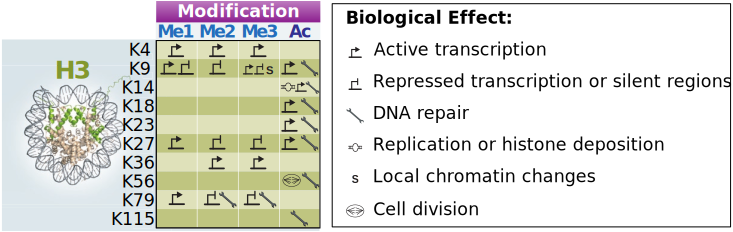
\includegraphics[width=0.8\textwidth]{lall_1111_histone_modifications}
\caption[Main histone modifications on lysines of histone H3]{\textbf{Main histone modifications on lysines of histone H3.} The tail of the histone H3 undergo post-translation modifications which are associated to chromatin remodeling. Different modifications at different locations of the H3's tail have contrasting effects such as transcription initiation or repression. \emph{Source: Lall et al.}\cite{lall2007} (modified to fit thesis format and/or clarify key points).}
\label{fig:lall_histone_modifications}
\end{figure}

% Chromatin structure provides cell-specificity
The fact that different parts of the genome can be open and closed at different times, allowing a specific set of genes to be expressed under different cell conditions, is one of the main mechanisms in which we are able to observe such a high number of different cells despite the fact that they carry the same underlying genetic information. The Figure~\ref{fig:lodish_open_closed_chromatin} shows a graphical example of two cells at different stages of commitment. Although the genomic region depicted is the same for these two cells, one present a closed chromatin structure, while the other present an open chromatin structure. The closed chromatin observed for the long-term hematopoietic stem cell (Figure~\ref{fig:lodish_open_closed_chromatin}a) does not allow the gene ATF3 to be transcribed, while the open chromatin structure present in the monocyte cell (Figure~\ref{fig:lodish_open_closed_chromatin}b) does allow the expression of ATF3 gene, since the transcription factors and transcription machinery are able to access that region and start the transcription process.

% Figure - Open versus closed chromatin
\begin{figure}[h!]
\centering
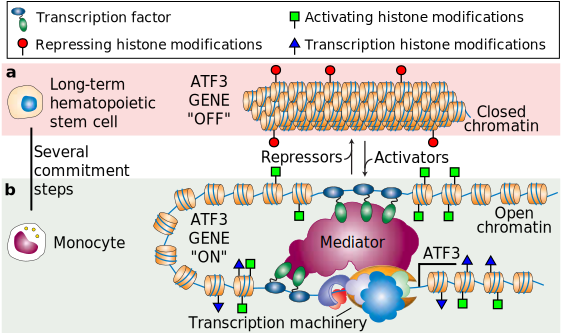
\includegraphics[width=0.8\textwidth]{lodish_461_open_closed_chromatin}
\caption[Open \emph{versus} closed chromatin]{\textbf{Open \emph{versus} closed chromatin.} Transription factor binding sites are cell-condition specific. This means that the same genomic locus might be accessible in a particular cell condition and not accessible in other condition. Such chromatin dynamics, which are modulated by genetic and epigenetic factors such as histone modifications, are responsible for the specialization of cells in performing the particular tasks required by the tissues they are located. This figure shows a graphical example of a locus (ATF3 gene) which is (\textbf{a}) closed in long-term hematopoietic stem cells (\textbf{b}) open in monocytes. Monocytes are a product of multiple specialization steps in hematopoietic stem cells. In this figure we show histone modifications which marks open/closed chromatin and proximal/distal regulatory regions. \emph{Source: Lodish et al.}\cite{lodish2007} (modified to fit thesis format and/or clarify key points).}
\label{fig:lodish_open_closed_chromatin}
\end{figure}

%%%%%%%%%%%%%%%%%%%%%%%%%%%%%%%%%%%%%%%%%%%%%%%%%%%%%%%%%%%%%%%%%%%%%
% Section: Next-Generation Sequencing Methods
%%%%%%%%%%%%%%%%%%%%%%%%%%%%%%%%%%%%%%%%%%%%%%%%%%%%%%%%%%%%%%%%%%%%%
\section{Next-Generation Sequencing Methods}
\label{sec:ngs.methods}

% Introduction
Recently, novel DNA sequencing platforms have enabled the sequencing of a very large number of DNA fragments (up to a few billions) on one single assay with a significant decrease in cost and complexity~\cite{hayden2014}. However, although these techniques are able to sequence a very large number of DNA fragments per single execution; these fragments must be small (usually up to hundreds of bp). We refer to these novel sequencing platforms as next-generation sequencing (NGS)~\cite{shendure2008}. Since the development of the first NGS technologies~\cite{tucker2009}, they have been constantly improving. A complete discussion on NGS can be found at Rusk et al.~\cite{rusk2010}.

% Adapt old techniques
The emergence of NGS and its constant technological improvements have enabled the revisiting of traditional biological assays to investigate regulatory elements (described in Section~\ref{sec:eukaryotic.regulation}) using the cell-specific chromatin dynamics context (described in Section~\ref{sec:chromatin.dynamics}). On revisiting such methods, their protocols could be adapted in order to fit the NGS technologies, which enables them to be performed in a genome-wide manner. Such large-scale analysis has potential to reveal the high-dimensional relationships between regulatory elements. NGS-based assays have enabled multiple current research progress, which unraveled the regulatory mechanisms linked to conditions, such as cell differentiation or the onset of diseases, of multiple cells.

% This section
In this section we will describe the following techniques: (1) Chromatin immunoprecipitation followed by NGS (ChIP-seq; Section~\ref{sec:chip.seq}) and (2) DNase I footprinting followed by NGS (DNase-seq; Section~\ref{sec:dnase.seq}).

%%%%%%%%%%%%%%%%%%%%%%%%%%%%%%%%%%%%%%%%%%%%%%%%%%%%%%%%%%%%%%%%%%%%%
% Subsection: ChIP-seq
%%%%%%%%%%%%%%%%%%%%%%%%%%%%%%%%%%%%%%%%%%%%%%%%%%%%%%%%%%%%%%%%%%%%%
\subsection{ChIP-seq}
\label{sec:chip.seq}

% ChIP-seq introduction
The ChIP-seq technique~\cite{johnson2007} consists on fetching target DNA-bound proteins and further sequencing of the DNA fragments fetched using NGS techniques. These target proteins can be, for instance, transcription factors or histones with a particular post-translational modification. This allows the genome-wide identification of the genomic regions in which a target protein is bound within a single experimental execution. When applied to a target transcription factor, the ChIP-seq experiment allows us to identify the transcription factor binding sites. When applied to histones with particular post-translational modification, the ChIP-seq experiment allows us to identify the genomic regions in which these modified histones occur, and therefore make inferences on that region's particular chromatin structure.

% ChIP-seq process
The ChIP-seq protocol starts by isolating the nuclei of cells and breaking them in order to access the genomic material (chromatin). The isolated genomic material is cross-linked in order to preserve all protein-DNA binding events. Next, the crosslinked chromatin is sheared into approximately $200$ bp DNA fragments with any massive DNA shearing procedure. Afterwards, the chromatin lysate is treated with an antibody that targets a particular protein of interest. The solution is then immunoprecipitated. In this procedure, we fetch only the sheared chromatin fragments that contains the protein of interest. The immunoprecipitated solution is separated and washed in order to keep only the DNA fragments. Then, these DNA fragments are sequenced using a NGS technique. It is important to mention that only the beginning of the fetched DNA fragments are sequenced ($50$--$100$ bp) by NGS techniques. Such process is depicted in Figure~\ref{fig:gusmao_chipseq}a--c.

% ChIP-seq process - genomic signal
The sequenced DNA fragments (termed ``reads'') can be mapped back into the reference genome using massive string alignment algorithms (Figure~\ref{fig:gusmao_chipseq}d), which are developed specially for mapping short DNA reads (length of $50$--$100$ bp) into a big reference genome (human genome length is \approxy$3.1$ billion bp). Such demanding computational problem is considered a solved problem and there are many available algorithms such as Bowtie~2~\cite{langmead2012} or the Burrows-Wheeler Aligner (BWA)~\cite{li2009b}. Given these aligned reads, we are able to generate a genomic signal by calculating the overlap between these reads at every genomic coordinate, i.e. every bp of the genome (Figure~\ref{fig:gusmao_chipseq}e). Nevertheless, since only the first $50$--$100$ bp of the fetched fragments are sequenced, they need to be extended to the approximate total size of the fetched fragments (approximately $200$ bp). This extension step reflects the fact that the protein can be bound to virtually any location of the fetched DNA fragment.

% ChIP-seq process - enrichment
Finally, we are able to identify the binding locations of the target protein by identifying regions significantly enriched with the genomic signal (Figure~\ref{fig:gusmao_chipseq}f). This is also a computationally demanding problem which was solved with the development of modern genomic peak-calling algorithms such as the model-based analysis for ChIP-seq (MACS)~\cite{zhang2008}. Since the ChIP-seq signal has a low resolution, i.e. it is smoothed given the fact that we have to extend the aligned reads, the target protein is considered to be likely bound anywhere within the called peaks.

% Figure - ChIP sequencing experimental technique (ChIP-seq)
\begin{figure}[h!]
\centering
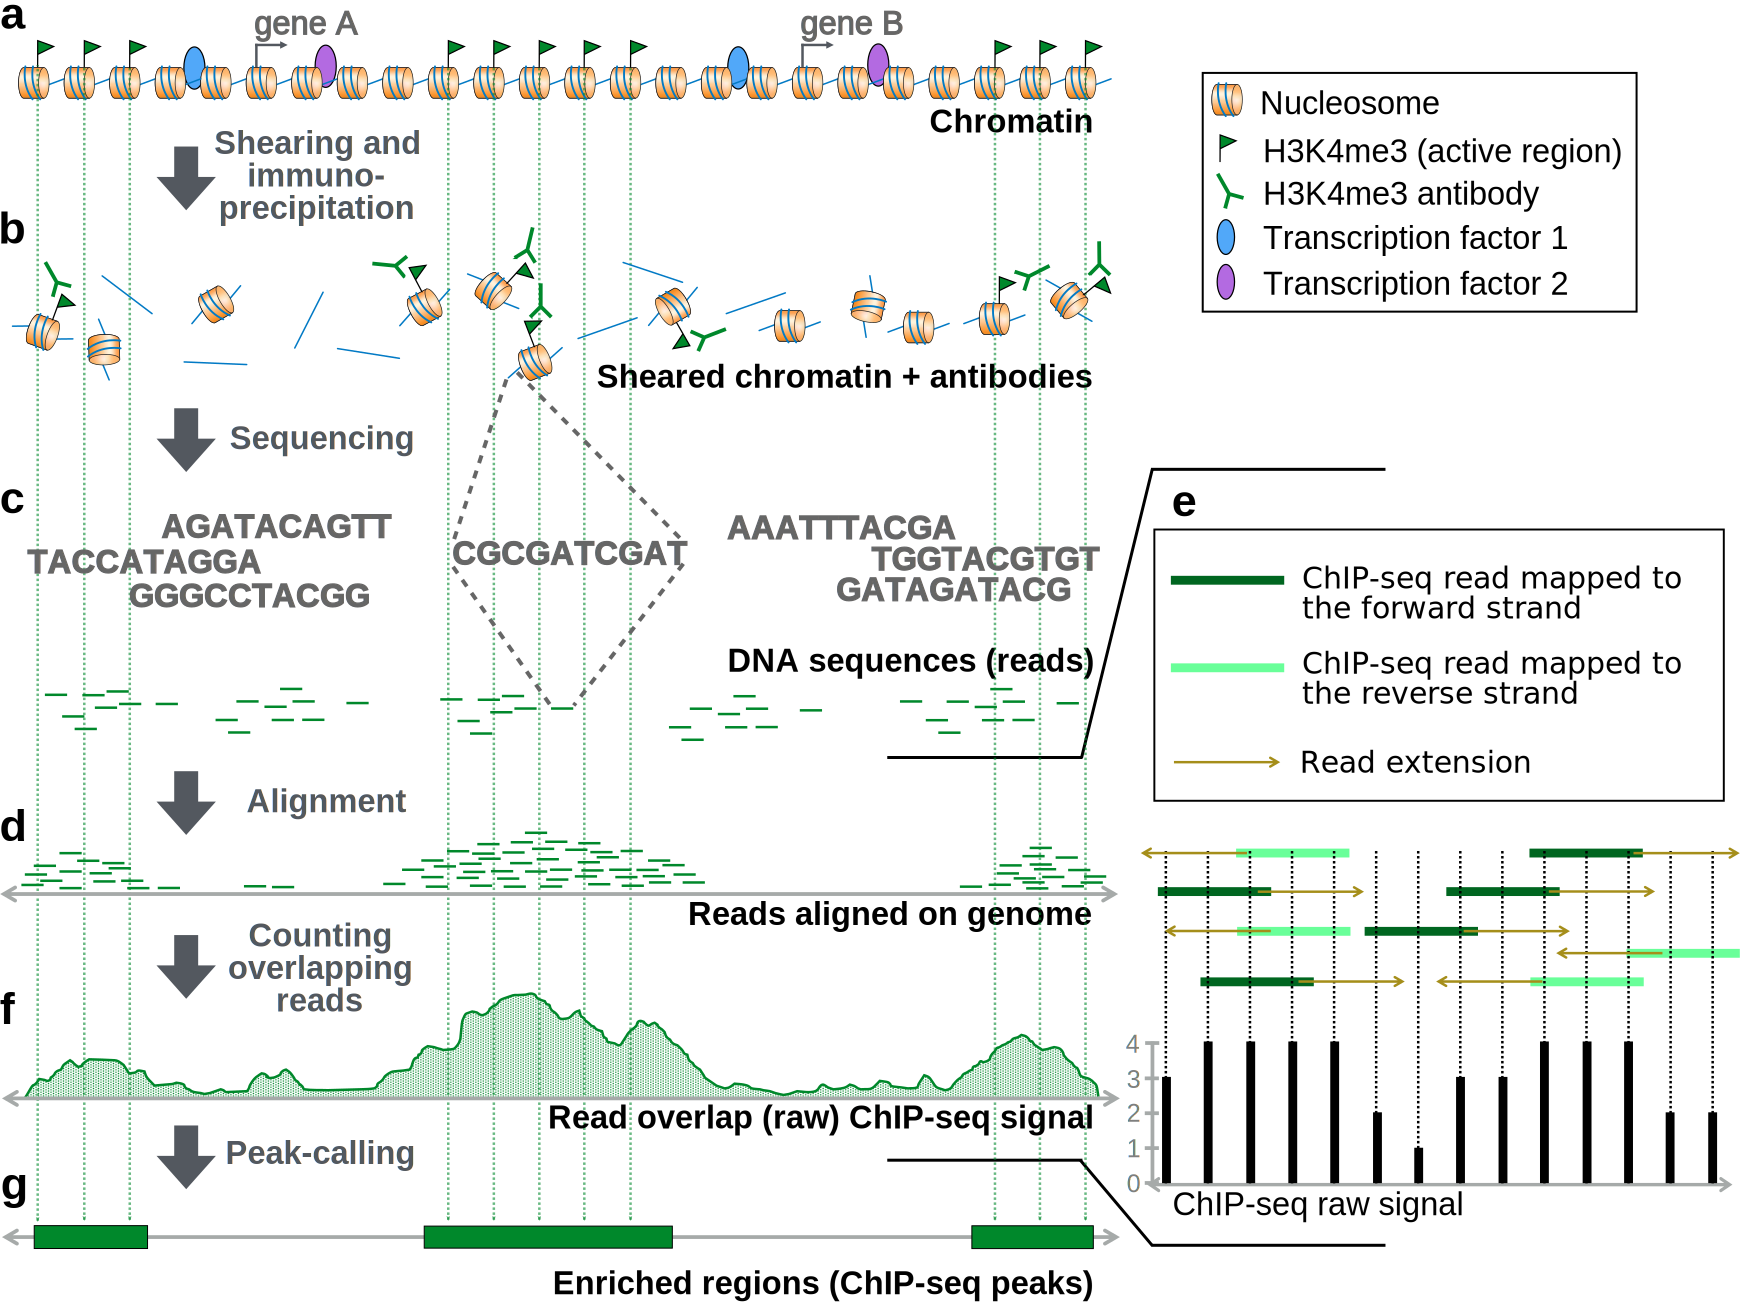
\includegraphics[width=0.99\textwidth]{gusmao_chipseq}
\caption[ChIP sequencing experimental technique (ChIP-seq)]{\textbf{ChIP sequencing experimental technique (ChIP-seq).} (\textbf{a}) The protocol starts by fetching the chromatin from multiple cells. Such chromatin is cross-linked to preserve all protein-DNA interactions. (\textbf{b}) The cross-linked chromatin is sheared and treated with antibodies that target a particular protein of interest. The antibodies will bind the target-protein and the chromatin fragments bound by these antibodies can be recovered (immunoprecipitated). (\textbf{c}) The DNA fragments are sequenced using NGS-based techniques. Only the first $50$--$100$ bp of the \approxy$200$ bp fragments are sequenced. (\textbf{d}) The sequenced DNA fragments (reads) are mapped back into the reference genome using an alignment algorithm. (\textbf{e}) A genomic signal can be generated by counting the overlap of the extended mapped reads. The reads are extended to match their original immunoprecipitated fragment length of \approxy$200$ bp. (\textbf{f}) The resulting genomic signal is enriched, i.e. present peaks, in the locations where the target protein is likely bound in the genome. (\textbf{g}) We can search for regions enriched with the ChIP-seq signal, which are the putative regions in which the target-protein is binding in the genome, using a peak-calling algorithm.}
\label{fig:gusmao_chipseq}
\end{figure}

%%%%%%%%%%%%%%%%%%%%%%%%%%%%%%%%%%%%%%%%%%%%%%%%%%%%%%%%%%%%%%%%%%%%%
% Subsection: DNase-seq
%%%%%%%%%%%%%%%%%%%%%%%%%%%%%%%%%%%%%%%%%%%%%%%%%%%%%%%%%%%%%%%%%%%%%
\subsection{DNase-seq}
\label{sec:dnase.seq}

% DNase-seq intro
The DNase-seq technique~\cite{crawford2004,sabo2004a} consists in the observation of the DNA digestion by a certain cleavage agent able to break the DNA molecule. The cleavage agent used in this method is the enzyme deoxyribonuclease I (DNase I). The rationale of this method is that the DNase I enzyme can cleave the DNA in regions where it is accessible (i.e. open chromatin). Furthermore, within open chromatin regions, the DNase I enzyme will only be able to cleave the DNA at protein-free regions, leaving ``footprint marks'' that can be traced back as DNA-bound regulatory proteins.

% DNase-seq process - dnase I digestion & sequencing
The DNase-seq protocol starts by isolating the nuclei of cells and breaking them in order to access the genomic material (chromatin). The isolated genomic material will be treated with optimal concentrations of DNase~I, which will cleave the chromatin at random accessible positions. These accessible positions are the chromatin regions in which the DNA is open (i.e. not fully wrapped around the histone complexes) and protein-free (i.e. not being bound by proteins such as transcription factors). Such cleaved DNA fragments can be isolated and sequenced using the same algorithms as described for the ChIP-seq procedure (Section~\ref{sec:chip.seq}). Such process is depicted in Figure~\ref{fig:gusmao_dnaseseq}a--e.

% DNase-seq process - genomic signal
Then, we are able to create a genomic signal by counting the number of overlapping reads at every genomic position. In the DNase-seq case, we only count the $5^{\prime}$ position of the reads, since that is the position in which the DNase~I enzyme has cleaved the DNA and indicates an open chromatin region (Figure~\ref{fig:gusmao_dnaseseq}f). The resulting genomic signal will represent a nucleotide resolution map of the open chromatin positions within the whole genome.

% DNase-seq process - enriched regions and footprints
Finally, we are able to detect the DNase-seq enriched regions by using algorithms specially designed for such purpose such as the F-seq~\cite{boyle2008b} (Figure~\ref{fig:gusmao_dnaseseq}g). Each region enriched with DNase-seq reads -- termed DNase I hypersensitivity sites (DHSs) -- are composed of several DNase-seq signal peaks. Note that the depletions within two of these nucleotide resolution peaks are indicative of a region which the DNase~I enzyme could not access because there was probably a protein binding in that region. These depleteions between two peaks are called ``footprints'' and the identification of these regions gives us a genome-wide map of putative active transcription factor binding sites.

% Figure - DNase I sequencing experimental technique (DNase-seq)
\begin{figure}[h!]
\centering
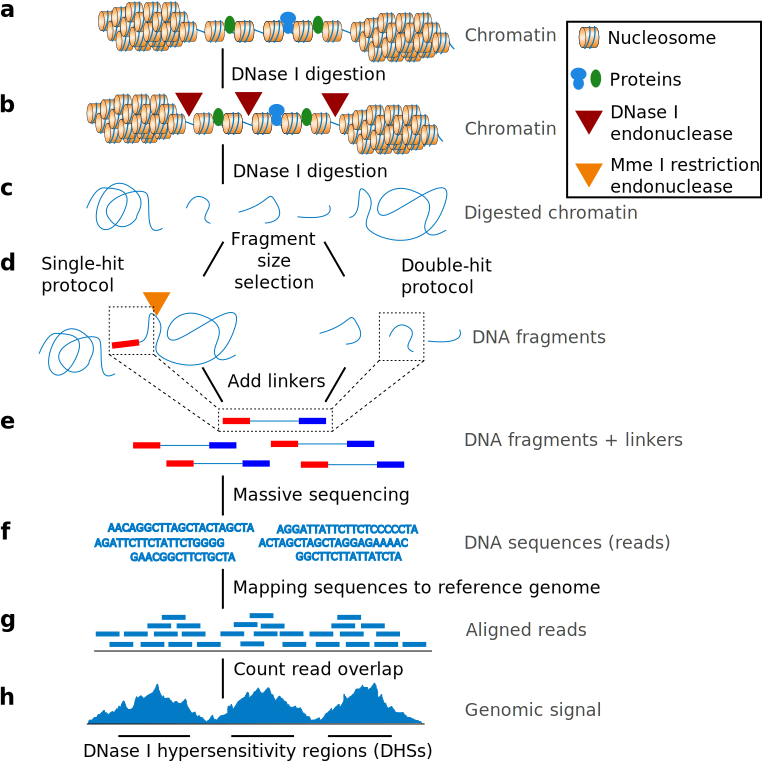
\includegraphics[width=0.8\textwidth]{gusmao_dnaseseq}
\caption[DNase I sequencing experimental technique (DNase-seq)]{\textbf{DNase I sequencing experimental technique (DNase-seq).} (\textbf{a}) The protocol starts by fetching the chromatin from multiple cells. (\textbf{b}) The chromatin is treated with optimal levels of DNase I enzyme, which will cleave the chromatin in accessible sites. These accessible sites are the ones in which the chromatin is open and is not being bound by transcription factors. (\textbf{c}) After the DNase I digestion we have multiple fragments of sheared chromatin. The ends of these fragments are isolated. (\textbf{d}) The isolated DNA fragments' ends are sequenced using NGS-based techniques. (\textbf{e}) The aligned DNA sequences are mapped back into the reference genome. (\textbf{f}) A signal can be generated by counting the overlap of the mapped DNA sequences. Only the first bp (i.e. $5^{\prime}$ bp) of the aligned read is count during the creation of the overlap signal. This is a reflection of the fact that we are interested in the positions in which the DNase I enzyme has cleaved the DNA. (\textbf{g}) The resulting read overlap signal will exhibit peaks in the open chromatin (accessible to DNase I) regions. (\textbf{h}) Regions with high concentration of DNase-seq reads are termed DNase I hypersensitivity sites (DHSs). Each of these regions are characterized by a number of depletions between peaks, which represent transcription factor footprints.}
\label{fig:gusmao_dnaseseq}
\end{figure}

% DNase-seq vs ChIP-seq
It is important to point the differences between DNase-seq and ChIP-seq. In the DNase-seq method, we determine the binding of any protein in the region being analyzed, without knowing which protein is binding; however in ChIP-seq we only determine the binding of a particular target protein with a known antibody in the region of interest. Furthermore, while the DNase-seq can provide the precise protein binding location, the ChIP-seq tells us an approximated region for the binding of the target protein, since the protein can be virtually anywhere within the \approxy$200$ bp immunoprecipitated fragments. The selection of the technique to use depends mainly on the experimental design and should consider these important details.

%%%%%%%%%%%%%%%%%%%%%%%%%%%%%%%%%%%%%%%%%%%%%%%%%%%%%%%%%%%%%%%%%%%%%
% Section: Active Binding Site Detection
%%%%%%%%%%%%%%%%%%%%%%%%%%%%%%%%%%%%%%%%%%%%%%%%%%%%%%%%%%%%%%%%%%%%%
\section{Active Binding Site Detection}
\label{sec:active.binding.site.detection}

% This section
In this section we define the problem we are going to address in this thesis - the computational identification of transcription factor binding sites. First, we define the problem (Section~\ref{sec:problem.definition}). Then, we make a brief discussion on why this is an important subject of study (Section~\ref{sec:significance}). In sequence, we discuss a computational sequence-based method for the identification of transcription factor binding sites and its inability to differentiate between active and inactive binding sites (Section~\ref{sec:computational.sequence.method}). Such discussion provides some insight on the difficulty of active transcription factor binding site identification. Finally, we show how biological experimental assays such as DNase-seq and ChIP-seq can be used to provide information necessary to differentiate active from inactive transcription factor binding sites (Section~\ref{sec:grammar.tfbs}).

%%%%%%%%%%%%%%%%%%%%%%%%%%%%%%%%%%%%%%%%%%%%%%%%%%%%%%%%%%%%%%%%%%%%%
% Subsection: Problem Definition
%%%%%%%%%%%%%%%%%%%%%%%%%%%%%%%%%%%%%%%%%%%%%%%%%%%%%%%%%%%%%%%%%%%%%
\subsection{Problem Definition}
\label{sec:problem.definition}

% Introduction to the problem
In Section~\ref{sec:eukaryotic.regulation}, we presented an overview of main features regarding eukaryotic gene regulation. One of the main features presented are the transcription factors, which are proteins that bind to specific genomic regions called transcription factor binding sites. Furthermore, the transcription factors binding process is highly dynamic and varies between different cells and cellular conditions given the chromatin dynamics context (Section~\ref{sec:chromatin.dynamics}). Such dynamic regulatory process collaborates with the orchestration of proper spatial and temporal expression of genes. Therefore, the identification of such regulatory elements is crucial to understand regulatory networks driving multiple cellular processes and the onset of diseases which manifest due to regulatory network disruption. Given that, we can formally define the problem we are addressing in this work:

\vspace{0.5cm}
\noindent
\textbf{Active Binding Site Detection Problem:} \emph{For a given cell's genome, find all putative genomic regions (termed transcription factor binding sites) in which there are proteins (termed transcription factors) binding, playing a specific regulatory role in the gene expression of the cell.}
\vspace{0.45cm}

% Different approaches - system-focused
The problem of active binding site detection has a few variants, depending mainly on the specific goals of research analyses. On the one hand, system-focused analyses require the identification of a few target binding sites. In this case, there is \emph{a priori} knowledge on the particular regulatory players involved at the particular mechanism being studied. Such problem is usually addressed by biological experimental assays such as ChIP-seq (Section~\ref{sec:chip.seq}) for the target transcription factors if interest.

% Different approaches - system-exploratory
On the other hand, system-exploratory analyses require a genome-wide map of all putative transcription factor binding sites that are being bound by proteins at a particular cell condition. In this case the researchers are interested in a genome-wide map of all putative active binding sites in order to perform various further inferences on the regulatory dynamics of the system under study. In this case, the problem can be addressed by biological techniques such as DNase-seq (Section~\ref{sec:dnase.seq}).

%%%%%%%%%%%%%%%%%%%%%%%%%%%%%%%%%%%%%%%%%%%%%%%%%%%%%%%%%%%%%%%%%%%%%
% Subsection: Significance
%%%%%%%%%%%%%%%%%%%%%%%%%%%%%%%%%%%%%%%%%%%%%%%%%%%%%%%%%%%%%%%%%%%%%
\subsection{Significance}
\label{sec:significance}

% Importance of the problem - examples
As previously mentioned, the identification of regulatory elements is a very important task, since they are the key players on most regulatory mechanisms. The subject under study can be an individual cell type's regulatory landscape or the mechanisms behind a system of two or more different cell types. There are a great number of studies that benefited from the proper identification of active binding sites. Recent studies, that uses NGS-based experimental techniques coupled with proper computational frameworks, have particularly provided multiple insights on a different range of mechanisms such as cell differentiation and understanding the onset of diseases. For instance, studies were able to: (1) unravel cellular differentiation processes~\cite{lin2015,tsankov2015}; (2) unravel disease mechanisms~\cite{schaub2012,vernot2012,charos2012}; (3) perform gene expression prediction and high-order functional analyses~\cite{yip2012,whitfield2012,natarajan2012} and (4) understand other cellular regulatory elements such as long noncoding RNAs~\cite{tilgner2012,banfai2012}. In summary, the identification of active transcription factor binding sites is important because of its broad impact on many other cellular processes.

% Problem's issues
However, there are many issues that makes this a challenging problem. First, the regulatory landscape is cell condition-specific, i.e. each cell undergoing a specific stage/process/condition/stimulus contains a different set of regions accessible by transcription factors. Also, there are over $1,500$ known transcription factors, each of which can bind to the DNA directly or by being recruited (such as co-activators). The possible combinatorial binding framework makes it very hard to unravel regulatory regions on a transcription factor-wise approach. Furthermore, some transcription factors bind in a very dynamic manner, which makes hard to interpret a particular snapshot of the regulatory landscape captured at a specific moment of the cell's lifetime.

%%%%%%%%%%%%%%%%%%%%%%%%%%%%%%%%%%%%%%%%%%%%%%%%%%%%%%%%%%%%%%%%%%%%%
% Subsection: Computational Sequence-Based Method
%%%%%%%%%%%%%%%%%%%%%%%%%%%%%%%%%%%%%%%%%%%%%%%%%%%%%%%%%%%%%%%%%%%%%
\subsection{Computational Sequence-Based Methods \& Limitations}
\label{sec:computational.sequence.method}

% Introduction
With the increasing demand for methods that are able to analyze the whole genome and given the fact that biological experimental assays are highly technical and time-consuming, some computational DNA sequence-based approaches were developed in order to aid the genome-wide search of transcription factor binding sites.

% String matching
One of the first sequence-based computational approaches consisted on a string-matching algorithm that used information regarding the transcription factor's DNA sequence binding affinity (i.e. transcription factor DNA motif) to build mathematical models that could be used to search for similar sequences in the genome. Such algorithms are called ``motif matching''~\cite{stormo2000}. The transcription factor binding sites predicted using sequence-based computational methods are called motif-predicted binding sites (MPBSs).

% Motif matching disadvantages
Some versions of computational sequence-based method have very reasonable accuracy rates and their low computational complexity makes it much easier to apply than the highly-technical and time-consuming biological assays~\cite{mathelier2013}. However, this technique has a major disadvantage: it is unable to identify active binding sites, i.e. binding sites that are actually being bound by proteins at a specific cellular condition. This happens because computational sequence-based methods rely solely on the DNA sequence affinity of proteins. However, the DNA sequence is the same between different cells for a particular organism; independent of cell type, cellular condition, life stage, stimuli response, and others. The key factor which allows different cells with the same genetic material to express a different set of proteins is the chromatin structure. Therefore, computational sequence-based methods are not able to capture the active (cell-specific) binding sites.

% Motif matching disadvantages
In practice, the fact that sequence-based computational approaches are unable to identify active binding sites is usually expressed as a very high number of false positive predictions, which represent the transcription factor binding sites which are not being accessed in a particular cellular condition. The Figure~\ref{fig:gusmao_motif_match_problem} exemplifies this issue. A motif matching tool was applied in a small genomic region using $520$ transcription factors affinity representations with a conservative threshold to accept binding site hits. The result shows more than $3,000$ motif-predicted binding sites on a $3,000$ bp region, which absolutely does not correspond to any possible biological regulatory model.

% Figure - Main problem of computational sequence-based methods
\begin{figure}[h!]
\centering
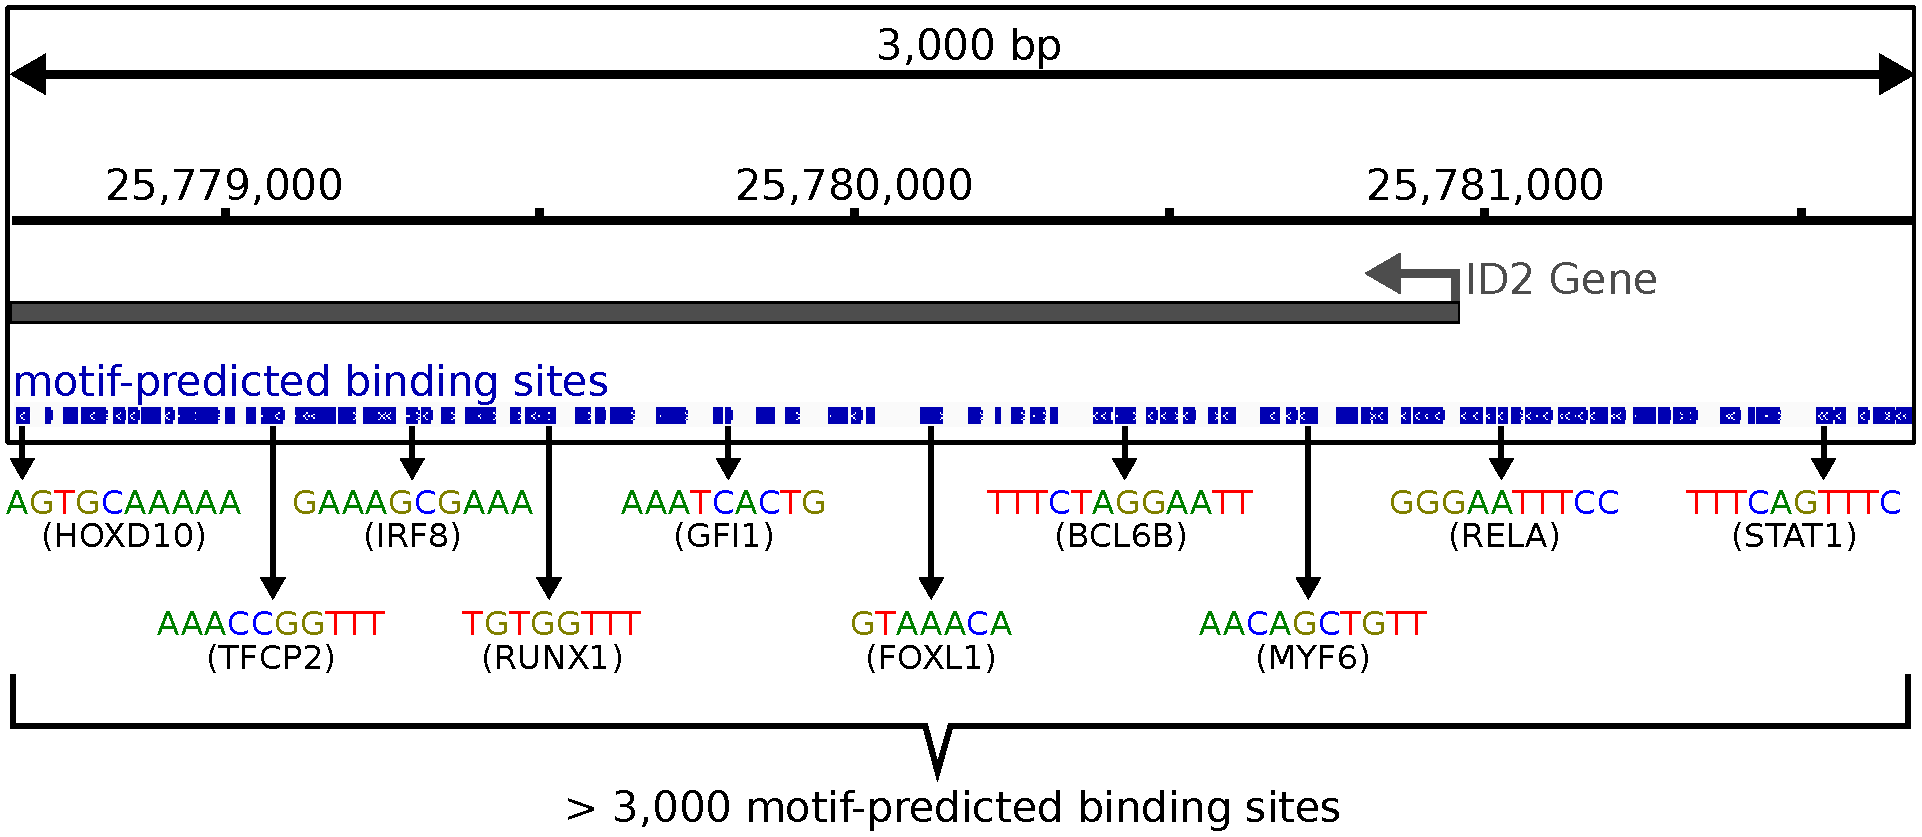
\includegraphics[width=0.95\textwidth]{gusmao_motif_match_problem}
\caption[Main problem of computational sequence-based methods]{\textbf{Main problem of computational sequence-based methods.} The motif matching tool FIMO~\cite{grant2011} was applied in a $3,000$ bp genomic region using $520$ transcription factor DNA sequence binding affinity models and resulted in more than $3,000$ motif-predicted binding sites. Such biologically impossible scenario exemplifies the fact that sequence-based computational approaches (such as motif matching) are unable to identify active binding sites.}
\label{fig:gusmao_motif_match_problem}
\end{figure}

%%%%%%%%%%%%%%%%%%%%%%%%%%%%%%%%%%%%%%%%%%%%%%%%%%%%%%%%%%%%%%%%%%%%%
% Subsection: Grammar of Active Transcription Factor Binding Sites
%%%%%%%%%%%%%%%%%%%%%%%%%%%%%%%%%%%%%%%%%%%%%%%%%%%%%%%%%%%%%%%%%%%%%
\subsection{Grammar of Active Transcription Factor Binding Sites}
\label{sec:grammar.tfbs}

% Introduction and ChIP-seq
In order to make predictions of active transcription factor binding sites, we must use chromatin dynamics information that provides the required cell-specificity. Such information can be obtained with the biological assays discussed in Section~\ref{sec:ngs.methods}. The most straightforward approach to obtain active transcription factor binding sites is to perform ChIP-seq on the target transcription factors of interest. Such assay will provide all transcription factor binding sites for such target transcription factors with a very good accuracy and reasonable resolution. However, using ChIP-seq directly for transcription has a few limitations. First, the ChIP-seq relies on the quality of the antibody used on the immunoprecipitation step. There are many transcription factors in which the antibodies do not work properly or do not work at all. Second, if the experimental design relies on the identification of a very small number of transcription factors (system-focused experiment design) then ChIP-seq for transcription factors might be a good choice; however, if one is interested in a higher number of transcription factors (system-exploratory experiment design), the number of transcription factor ChIP-seq assays makes the study very expensive and time consuming.

% Using open chromatin markers
Current research aims at identifying the greatest number of possible active transcription factor binding sites with the lowest possible number of experimental assays. Given the limitations of ChIP-seq for transcription factors for such system-focused experiment design, current studies rely on experimental open chromatin markers to narrow the search of active transcription factor binding sites. As previously discussed, the histone modifications, which can be obtained using ChIP-seq, mark regions in which the chromatin is open, and therefore accessible to transcription factors. Furthermore, the DNase-seq experimental assay provides open chromatin regions with a nucleotide resolution.

% Grammar of TFBSs
There is a well-known pattern that can be seen in genomic signals from DNase-seq and histone modification ChIP-seq. We will call this pattern the ``grammar of transcription factor binding sites''. This grammar, depicted in Figure~\ref{fig:gusmao_grammar_tfbs}, shows that transcription factor binding sites happen at depletions between two peaks of the DNase-seq signal. These regions with multiple DNase-seq peaks, which comprise a DNase I hypersensitivity site, occur within a depletion between two peaks of activating histone marks.

% Figure - Grammar of transcription factor binding sites
\begin{figure}[h!]
\centering
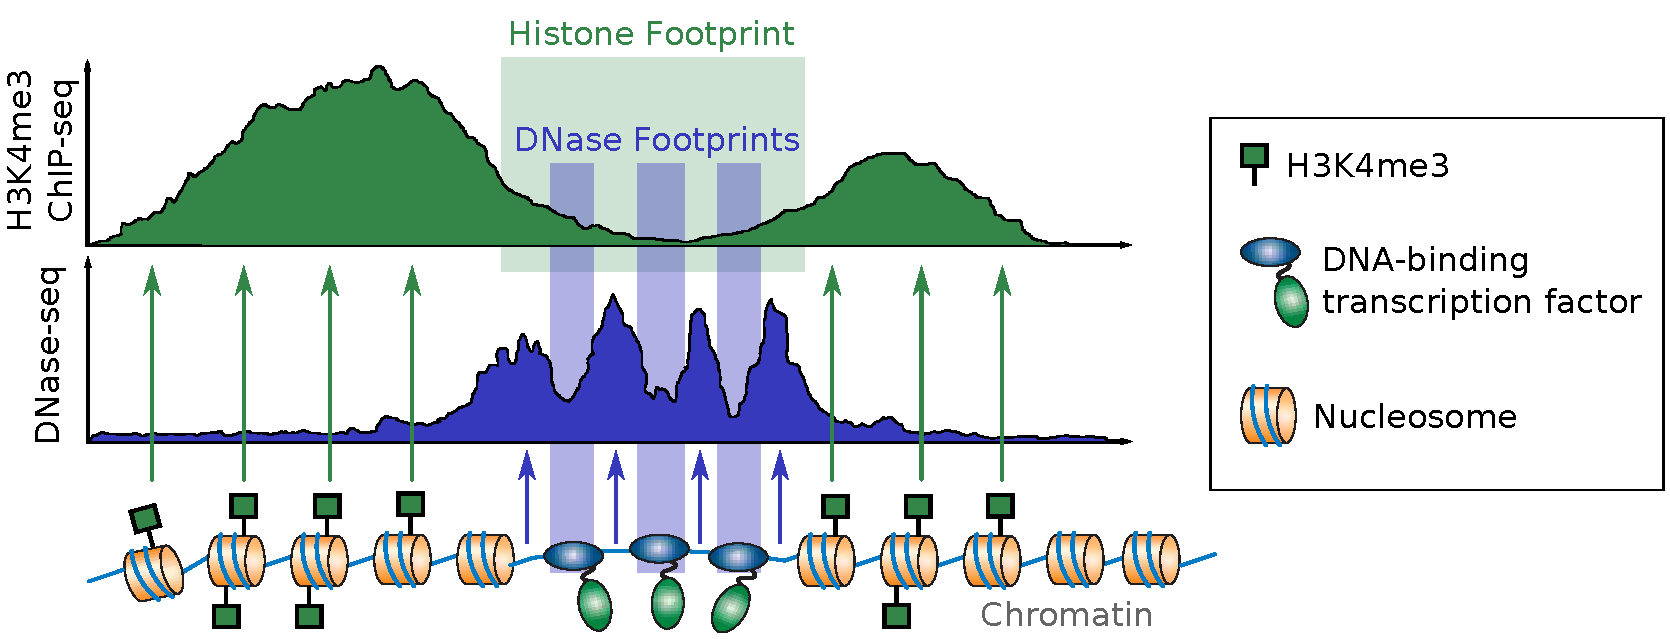
\includegraphics[width=0.85\textwidth]{gusmao_grammar_tfbs}
\caption[Grammar of transcription factor binding sites]{\textbf{Grammar of transcription factor binding sites.} In this figure we show examples of histone modification ChIP-seq and DNase-seq signals for a genomic region (top) and a graphical representation of the chromatin landscape within this region (bottom). We and others observed that there is a clear pattern regarding these signals and the transcription factor binding sites. Transcription factor binding sites happen at depletions between two peaks of the DNase-seq signal. Furthermore, these DNase-seq peaks, which determines an open chromatin region, happen at the depletion between two peaks of active histone modification marks.}
\label{fig:gusmao_grammar_tfbs}
\end{figure}

% Computational methods
Such pattern can be used in order to make better predictions of active binding sites, when compared to purely sequence-based methods (Section~\ref{sec:computational.sequence.method}). Furthermore, a complete map of all putative active transcription factor binding sites for a particular cell type can be obtained with a few assays (in the example of Figure~\ref{fig:gusmao_grammar_tfbs}, two assays: ChIP-seq for H3K4me3 and DNase-seq). However, the very high magnitude and complexity of the genomic signals generated with DNase-seq and histone modification ChIP-seq require special computational frameworks. Such computational frameworks which processes open chromatin NGS-based data gained popularity over the last years and can be used to address the problem of active transcription factor binding site prediction.

%%%%%%%%%%%%%%%%%%%%%%%%%%%%%%%%%%%%%%%%%%%%%%%%%%%%%%%%%%%%%%%%%%%%%
% Section: Computational Footprinting Methods
%%%%%%%%%%%%%%%%%%%%%%%%%%%%%%%%%%%%%%%%%%%%%%%%%%%%%%%%%%%%%%%%%%%%%
\section{Computational Footprinting Methods}
\label{sec:computational.footprinting.methods}

% This section
In this section we show how the state-of-the-art computational methods use the grammar of active transcription factor binding sites to provide predictions of active transcription factor binding sites. These computational methods are termed computational footprinting methods (Section~\ref{sec:method.definition}). Then, we will define the different types of computational footprinting methods (Section~\ref{sec:types.computational.footprinting.methods}) and briefly describe how these methods have been evaluated in the current literature (Section~\ref{sec:evaluation.computational.footprinting.methods}). Next, we show the main challenges on the identification of active transcription factor binding sites using computational footprinting approaches (Section~\ref{sec:current.challenges}). Finally, we close this section with a comprehensive literature review on published computational footprinting methods (Section~\ref{sec:literature.review}).

%%%%%%%%%%%%%%%%%%%%%%%%%%%%%%%%%%%%%%%%%%%%%%%%%%%%%%%%%%%%%%%%%%%%%
% Subsection: Method Definition
%%%%%%%%%%%%%%%%%%%%%%%%%%%%%%%%%%%%%%%%%%%%%%%%%%%%%%%%%%%%%%%%%%%%%
\subsection{Method Definition}
\label{sec:method.definition}

% Introduction
In this thesis we will focus on computational footprinting methods to address the problem of active transcription factor binding site prediction. In summary, the idea of using computational footprinting methods is to use the lowest number of assays possible in order to generate a robust active transcription factor binding site map. Therefore, the idea is to use experimental data that delineates open chromatin regions such as DNase-seq and ChIP-seq for histone modifications (instead of specific target transcription factors). We formalize the concept of computational footprinting method as follows:

\vspace{0.5cm}
\noindent
\textbf{Computational Footprinting Method:} \emph{A computational framework to analyze experimental open chromatin (NGS-based) data and create a genome-wide map of active transcription factor binding sites with the maximum resolution possible.}
\vspace{0.45cm}

% Discussion of definition - computational framework
We should clarify and dissect some parts of the above definition. First the term ``computational framework'' refers to a set of methods and algorithms used to process the open chromatin data and perform the prediction of putative active transcription factor binding sites. The input of these methods are the open chromatin signals, formally defined as a vector $\mathbf{x} = \langle x_1, \cdots, x_n \rangle$, where $n$ is the size of the genome in bp units and each $x_i \in \mathbb{R}$. We often refer to such a vector as a ``genomic signal''.

% Discussion of definition - Genome-wide prediction
Second, the ``genome-wide'' part assumes that the computational framework is capable of executing within a reasonable amount of time with data from all genomic coordinates. The open chromatin experimental assays provide genome-wide. However, in many occasions, the computational processing of such large amounts of data represents a bottleneck within the computational footprinting workflow. Therefore, effort has to be done on applying efficient data structures and algorithms with minimal computational complexity.

% Discussion of definition - map of active transcription factor binding sites
Third, the term ``map of active transcription factor binding sites'' refers to the output of these computational frameworks. This output should consist of multiple genomic regions, each of which starts and ends at particular genomic coordinates, which represents the putative active binding sites. More formally, the output of computational footprinting methods are simply a set $R = \{r_1, \cdots, r_m\}$ where $r_i = [u, v]$ represents an interval from the genomic coordinate $u$ to $v$ (including both), with length $v-u$ and $u<v$.

% Discussion of definition - maximum resolution possible
Fourth, the ``maximum resolution possible'' part refers to the fact that the predicted transcription factor binding site regions should be as close as possible, in terms of genomic position and predicted region's width, to the real transcription factor binding sites. In other words, the method should have a high spatial specificity. For instance, we could regard an entire open chromatin region (i.e. DNase I hypersensitivity site) as a putative region for transcription factors to bind. However, such region is large enough to include smaller genomic regions in which transcription factors do not bind or are not binding.

% Footprint score 
The simplest computational footprinting approach, termed ``the footprint score (FS)'', consists on sliding a window across the genome and evaluating the ratio between the number of reads (from a particular open chromatin experiment such as DNase-seq) inside the window and inside the flanking regions of the window (see Figure~\ref{fig:gusmao_computational_footprinting}). More formally, let $\mathbf{x} = \langle x_1, \cdots, x_n \rangle$ be a read overlap signal generated from DNase-seq experiment. The footprint score for a particular window represented as a genomic region $r_i = [u, v]$ can be evaluated as
\begin{equation}
  \label{eq:fs1}
  \text{FS}_{r_i} = \left(\frac{{n}^{C}_{r_i}+1}{{n}^{R}_{r_i}+1} + \frac{{n}^{C}_{r_i}+1}{{n}^{L}_{r_i}+1}\right),
\end{equation}
where
\begin{align}
  \label{eq:fs2}
  {n}^{C}_{r_i} &= \sum_{j=u}^{v} {x}_{j}, &
  {n}^{R}_{r_i} &= \sum_{j=v}^{2v-u} {x}_{j}, &
  {n}^{L}_{r_i} &= \sum_{j=2u-v}^{u} {x}_{j}.
\end{align}

% Footprint score
As depicted in Figure~\ref{fig:gusmao_computational_footprinting}, large positive numbers indicate that there are more reads (i.e. DNase I cleavage hits) in the core of the window than in the flanking region. On the other hand, low negative numbers indicate that there are more reads in the flanking region in comparison with the core. As a consequence of the grammar of active transcription factor binding sites, we regard the regions with low negative numbers as the predicted footprints.

% Conclusion
Simple approaches which relies on evaluating a score given a sliding window exemplifies the rationale behind computational footprinting methods. However, there are a number of different approaches to devise a computational footprinting framework.

% Figure - Simple example of computational footprinting
\begin{figure}[h!]
\centering
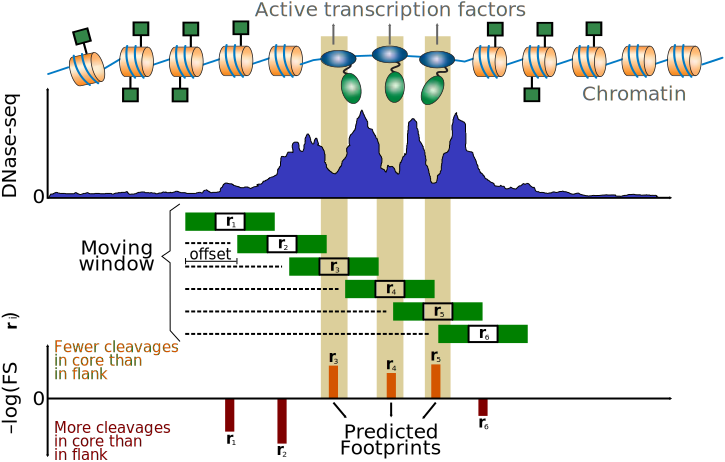
\includegraphics[width=0.70\textwidth]{gusmao_computational_footprinting}
\caption[Simple example of computational footprinting]{\textbf{Simple example of computational footprinting.} Depiction of a simple computational footprinting method which consists on sliding a window (termed $r_i$) composed of a core part (white box) and flanking regions (green box). The window, with a particular size, slides on the genome given a specific offset and evaluates a score. In the case of the footprint score shown in Equation~\ref{eq:fs1}, low negative values indicate footprints, which are putative active transcription factor binding site predictions.}
\label{fig:gusmao_computational_footprinting}
\end{figure}


%%%%%%%%%%%%%%%%%%%%%%%%%%%%%%%%%%%%%%%%%%%%%%%%%%%%%%%%%%%%%%%%%%%%%
% Section: Types of Computational Footprinting Methods
%%%%%%%%%%%%%%%%%%%%%%%%%%%%%%%%%%%%%%%%%%%%%%%%%%%%%%%%%%%%%%%%%%%%%
\subsection{Types of Computational Footprinting Methods}
\label{sec:types.computational.footprinting.methods}

% Segmentation vs site-centric methods
Computational footprinting methods are broadly categorized as: (1) segmentation methods and (2) site-centric methods. The main difference between these two groups of computational footprinting methods is that, while segmentation methods scans the genome for patterns of active transcription factor binding sites (such as the footprint score approach shown in Figure~\ref{fig:gusmao_computational_footprinting}); the site-centric approach uses \emph{a priori} predictions of transcription factor binding sites (such as motif-predicted binding sites, as shown in Section~\ref{sec:computational.sequence.method})) and use machine learning methods to classify these sites as true/false transcription factor binding sites.

% Segmentation methods
The rationale behind segmentation methods is to use NGS-based data to scan the genome for footprints. This approach generates a map of putative active binding sites without actually specifying the transcription factors that are binding these regions. Although further processing is necessary in order to identify which particular transcription factor bind to these putative binding sites; the advantage of such approach is that novel transcription factors or binding types can be detected. The Figure~\ref{fig:vierstra_5_segmentation_vs_sitecentric}a shows an example of the segmentation computational footprinting approach. The example shown in this figure is similar to the footprint score, shown in Figure~\ref{fig:gusmao_computational_footprinting}.

% Site-centric methods
On the other hand, site-centric methods start with putative binding sites obtained by using, for instance, a sequence-based prediction method such as motif matching (Section~\ref{sec:computational.sequence.method}). Then, experimental evidence around these \emph{a priori} predictions are gathered and classified generally using unsupervised machine learning methods. This approach leads to footprints for target transcription factors. The advantage of such approach is that we already know which transcription factors are binding to the correctly classified footprints. However, the disadvantage is that it depends on this \emph{a priori} transcription factor evidence, which is not always available. Furthermore, \emph{de novo} motif finding is not impossible on footprint predictions obtained with site-centric methods, while it is easily performed on the footprint predictions of segmentation approaches. The Figure~\ref{fig:vierstra_5_segmentation_vs_sitecentric}b provides a graphical representation of the site-centric approach. 

% Figure - Segmentation versus site-centric computational footprinting methods
\begin{figure}[h!]
\centering
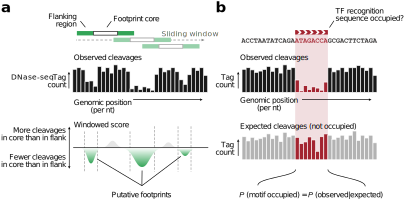
\includegraphics[width=0.99\textwidth]{vierstra_5_segmentation_vs_sitecentric}
\caption[Segmentation \emph{versus} site-centric computational footprinting methods]{\textbf{Segmentation \emph{versus} site-centric computational footprinting methods.} This figure show an example of each computational footprinting approach using DNase-seq data. Both methods tries to detect the grammar of active transcription factor binding sites described in Section~\ref{sec:grammar.tfbs}. (\textbf{a}) Graphical representation of the segmentation computational footprinting approach. In this case, the segmentation approach ``reads'' the DNase-seq signal as a time-series and tries to detect the footprint positions based on the footprint score. The output of this method are the genomic regions recognized as footprints given the grammar of active transcription factor binding sites. (\textbf{b}) The site-centric approach starts by detecting motif-predicted binding sites using sequence-based algorithms such as motif matching (Section~\ref{sec:computational.sequence.method}). Then, the DNase-seq signal around all motif-predicted binding sites is used to classify them as true/false binding sites. Such classification method will distinguish the motif-predicted binding sites that match the grammar of transcription factor binding sites (true MPBSs) from the ones that do not (false MPBSs). In this case, the true motif-predicted binding sites represent the footprint predictions.}
\label{fig:vierstra_5_segmentation_vs_sitecentric}
\end{figure}

%%%%%%%%%%%%%%%%%%%%%%%%%%%%%%%%%%%%%%%%%%%%%%%%%%%%%%%%%%%%%%%%%%%%%
% Section: Evaluation of Computational Footprinting Methods
%%%%%%%%%%%%%%%%%%%%%%%%%%%%%%%%%%%%%%%%%%%%%%%%%%%%%%%%%%%%%%%%%%%%%
\subsection{Evaluation of Computational Footprinting Methods}
\label{sec:evaluation.computational.footprinting.methods}

% Introduction
There is no well defined gold standard for the evaluation of footprinting methods. All works so far have used ChIP-seq of transcription factors in conjunction with motif-predicted binding sites as ground truth. Such method provides a straightforward scenario for the evaluation of computational footprinting methods. The idea behind such an evaluation approach is that the transcription factor ChIP-seq provides the cell-specificity and the motif-predicted binding sites provides a countable structure which can be used to extract some statistics. In the following we define such procedure.

% Procedure
In the ``ChIP-seq evaluation approach'' motif-predicted binding sites with ChIP-seq evidence (which can be, for instance, motif-predicted binding sites close to transcription factor ChIP-seq peak summits) are considered ``true'' TFBSs. On the other hand, motif-predicted binding sites without ChIP-seq evidence are considered ``false'' TFBSs. Every transcription factor prediction (i.e. footprint) that overlaps a true TFBS is considered a correct prediction (true positive -- TP) and every prediction that overlaps with a false TFBS is considered an incorrect prediction (false positive -- FP). Therefore, true negatives (TN) and false negatives (FN) are, respectively, false and true TFBSs without overlapping predictions. This is depicted on Figure~\ref{fig:gusmao_chipseq_evaluation}a.

% ROC curves and AUC
The contingency table (TPs, FPs, TNs and FNs) enables us to create receiver operating characteristic (ROC) curves, which describe the sensitivity increase as we decrease the specificity of the method (Figure~\ref{fig:gusmao_chipseq_evaluation}b). The area under the ROC curve (AUC) is a very good metric to rank computational footprinting methods. Furthermore, the contingency table also enables us to evaluate the area under the precision-recall curve (AUPR; Figure~\ref{fig:gusmao_chipseq_evaluation}c). This metric is indicated for problems with imbalanced datasets (distinct number of positive and negative examples)~\cite{davis2006,fawcett2006}. The AUC and AUPR metrics have been used in the literature to compare different computational footprinting methods in their ability to recover active transcription factor binding sites~\cite{pique2011,cuellar2012}.

% Figure - Evaluation of computational footprinting TODO
\begin{figure}[h!]
\centering
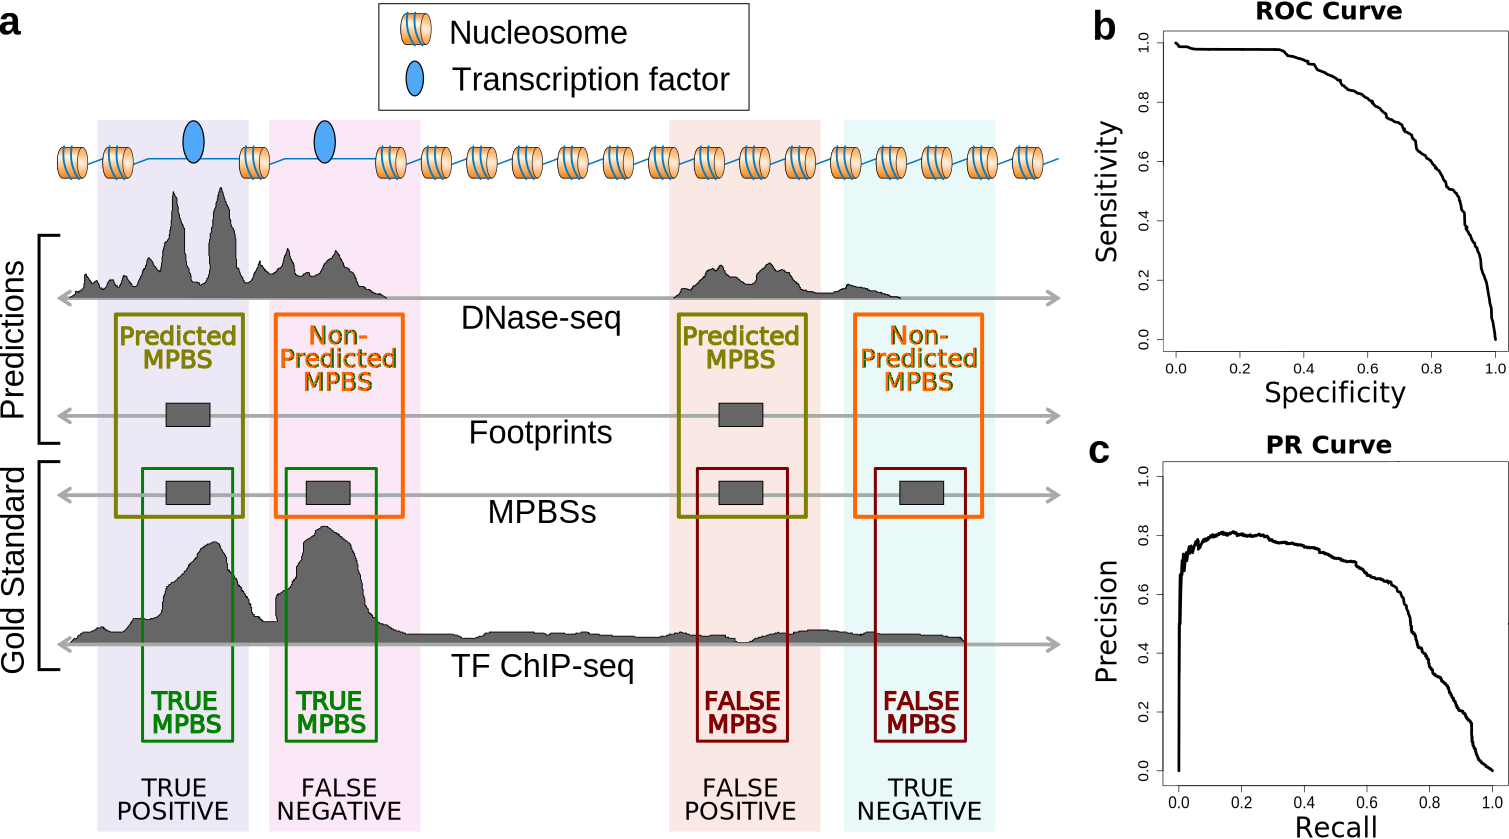
\includegraphics[width=0.9\textwidth]{gusmao_chipseq_evaluation}
\caption[Evaluation of computational footprinting]{\textbf{Evaluation of computational footprinting.} (\textbf{a}) In the ChIP-seq evaluation scheme, motif-predicted binding sites (MPBSs) for a particular transcription factor are considered true if they are within a ChIP-seq enriched region for that particular transcription factor. Otherwise, they are considered false MPBSs. By overlapping this information with footprint predictions from a particular computational footprinting method we are able to generate a contingency table with true positives, true negatives, false positives and false negatives. By ranking the motif-predicted binding sites based on the overlaping footprint's quality, we are able to create: (\textbf{b}) receiver operating characteristic (ROC) curves and (\textbf{c}) precision-recall (PR) curves. These structures can be used to rank the computational footprinting methods and evaluate their overall performance on identifying each transcription factor individually.}
\label{fig:gusmao_chipseq_evaluation}
\end{figure}

%%%%%%%%%%%%%%%%%%%%%%%%%%%%%%%%%%%%%%%%%%%%%%%%%%%%%%%%%%%%%%%%%%%%%
% Subsection: Current Challenges
%%%%%%%%%%%%%%%%%%%%%%%%%%%%%%%%%%%%%%%%%%%%%%%%%%%%%%%%%%%%%%%%%%%%%
\subsection{Current Challenges}
\label{sec:current.challenges}

% Signal treatment
It is known that open chromatin NGS-based genomic signals, such as DNase-seq and histone modification ChIP-seq, are very noisy and intrinsically complex. Most methods used some sort of smoothing approach to handle such complexity~\cite{pique2011,cuellar2012,sherwood2014,kahara2015}. Although a few attempts have been made to use these signals in their maximum possible resolution~\cite{boyle2011,sung2014}, not much attention was given to the proper processing methodology applied to these complex signals. The open chromatin NGS-based genomic signals can be affected by multiple artifacts stemming from either the biological protocol or the computational pre-processing steps. These artifacts were summarized recently by Meyer et al.~\cite{meyer2014}.

% Integrative approaches
Furthermore, none of the computational footprinting methods so far took advantage of the full (nucleotide resolution) spatial profile of all open chromatin NGS-based genomic signals. The current integrative approaches usually takes only the full spatial signal for only one of the signals, such as DNase-seq in the Centipede~\cite{pique2011} method; using other signals, such as histone modification ChIP-seq, as average read counts. The main reason discussed by most integrative approaches~\cite{pique2011,cuellar2012} is that it is hard to integrate signals which has a high degree of variation.

% asimmetry
Also, the observed average grammar of active transcription factor binding sites is not always symmetric~\cite{kundaje2012}. This means that one of the peaks in the peak-dip-peak pattern can be significantly shorter than the other and sometimes (as in the case of histone modifications) even nonexistent. Current computational footprinting methods, both segmentation and site-centric do not consider such intrinsic asimmetry~\cite{boyle2011,pique2011}.

% Lack of benchmark
Moreover, with the exception of a few studies~\cite{sherwood2014, yardimci2014, kahara2015}, comparative analyses evaluating footprinting methods analyzed only a few ($<12$) transcription factors. Also, a maximum of only four competing methods were evaluated using the same experiment design of a particular published study. In addition, the experiment design for evaluation of computational footprinting methods vary between different publications. Despite the importance of method evaluation~\cite{rusk2015}, there is a clear lack of benchmark data, evaluation standards and studies performing a comprehensive analysis of computational footprinting methods.

% Evaluation - ChIP-seq bias
Furthermore, when we consider the few studies that performed comparative analyses so far, all of them have used the ChIP-seq evaluation scheme as described in Section~\ref{sec:evaluation.computational.footprinting.methods}. This evaluation requires transcription factor ChIP-seq experiments to be carried out on the very same cells as the DNase-seq experiment and has a few caveats. First, transcription factor ChIP-seq peaks are also observed in indirect binding events~\cite{yardimci2014}. Second, they have a lower spatial resolution than DNase-seq. Therefore, false transcription factor binding sites might be regarded as true transcription factor binding sites by proximity to a real transcription factor binding site of a distinct transcription factor~\cite{cuellar2012,yardimci2014}.

% Bias-correction
Also, He et al.~\cite{he2014} showed that the DNase-seq sequence cleavage bias around transcription factor binding sites strongly affects the performance of a computational footprinting method (the footprint score -- FS -- as shown in Figure~\ref{fig:gusmao_computational_footprinting}) in a transcription factor-specific manner. Such bias stems from the fact that the DNase I enzyme, used in the DNase-seq experimental technique, prefers to bind to (and cleave) certain DNA $k$-mers than others. Such impact is depicted in Figure~\ref{fig:he_cleavage_bias}a. They also indicated several transcription factors, such as nuclear receptors and \emph{de novo} motifs found via computational footprinting~\cite{neph2012a}, where the DNase-seq profile resembles their sequence cleavage bias estimate (see Figure~\ref{fig:he_cleavage_bias}b and~c).

% Figure - Impact of DNase I cleavage bias on computational footprinting
\begin{figure}[h!]
\centering
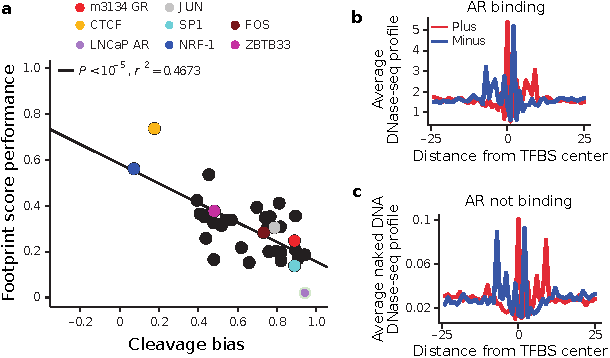
\includegraphics[width=0.75\textwidth]{he_5_cleavage_bias}
\caption[Impact of DNase I cleavage bias on computational footprinting]{\textbf{Impact of DNase I cleavage bias on computational footprinting.} (\textbf{a}) This graph shows the amount of sequence cleavage bias ($x$-axis) \emph{versus} the performance (AUC from the ChIP-seq evaluation approach) of the footprint score (FS) footprinting method. We can clearly observe that there is a strong negative correlation between these two variables. (\textbf{b}) Average DNase-seq signal profile around ChIP-seq peaks of the AR transcription factor in a cell type in which it is known that the AR transcription factor is being expressed. (\textbf{c}) Average DNase-seq signal profile around the same regions as in (b); however in this case the DNase-seq is from a naked DNA experiment, where all proteins were removed from the DNA. \emph{Source: He et al.}\cite{he2014} (modified to fit thesis format and/or clarify key points).}
\label{fig:he_cleavage_bias}
\end{figure}

% TF residence time
Besides the sequence cleavage bias, another experimental aspect affecting the computational analysis of DNase-seq is the residence time of transcription factor binding. Sung et al.~\cite{sung2014} showed that short-lived transcription factors display a lower DNase I cleavage protection pattern, i.e. low number of DNase-seq reads surrounding the footprint (see Figure~\ref{fig:sung_residence_time}). Such fleeting transcription factors are harder to detect than other transcription factors with longer residence time since their protection pattern is less pronounced.

% Figure - Transcription factor residence time
\begin{figure}[h!]
\centering
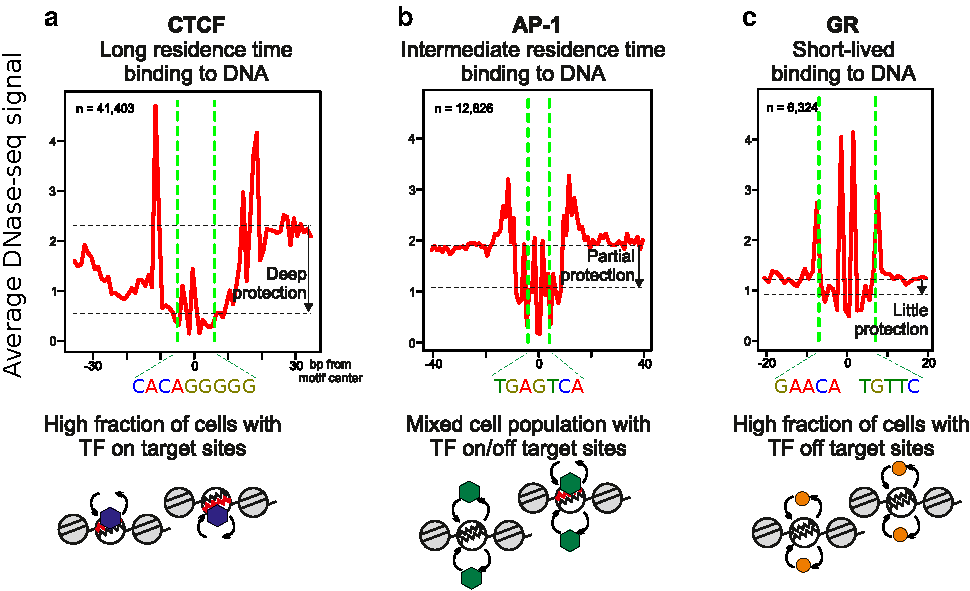
\includegraphics[width=0.8\textwidth]{sung_9_residence_time}
\caption[Transcription factor residence time]{\textbf{Transcription factor residence time.} This graphs depicts the average DNase-seq signal around transcription factor binding sites of transcription factors with: (\textbf{a}) long residence time -- CTCF; (\textbf{b}) intermediate residence time -- AP-1 (C-jun) and (\textbf{c}) short residence time -- GR. Sung et al.~\cite{sung2014} discuss that the width of the protection against the DNase I enzyme might be correlated with the residence time of the transcription factors in the DNA. \emph{Source: Sung et al.}\cite{sung2014} (modified to fit thesis format and/or clarify key points).}
\label{fig:sung_residence_time}
\end{figure}

%%%%%%%%%%%%%%%%%%%%%%%%%%%%%%%%%%%%%%%%%%%%%%%%%%%%%%%%%%%%%%%%%%%%%
% Section: Literature Review
%%%%%%%%%%%%%%%%%%%%%%%%%%%%%%%%%%%%%%%%%%%%%%%%%%%%%%%%%%%%%%%%%%%%%
\subsection{Literature Review}
\label{sec:literature.review}

% Introduction
A number of computational footprinting methods have been proposed. These methods used different open chromatin NGS-based experimental data sources, different algorithms and targets different experiment designs. Here, we will discuss the main published methods, providing a comprehensive literature review on computational footprinting methods.

%%%%%%%%%%%%%%%%%%%%%%%%%%%%%%%%%%%%%%%%%%%%%%%%%%%%%%%%%%%%%%%%%%%%%
% Section: Hesselberth et al.
%%%%%%%%%%%%%%%%%%%%%%%%%%%%%%%%%%%%%%%%%%%%%%%%%%%%%%%%%%%%%%%%%%%%%
\subsubsection{Hesselberth et al.}
\label{sec:hesselberth.2}

% Hesselberth (hesselberth2009) - method (Hesselberth)
One of the first attempts to create a computational footprinting method for DNase-seq data was performed by Hesselberth et al.~\cite{hesselberth2009}. In their study, they performed the DNase-seq experiment in the \emph{Saccharomyces cerevisiae} organism (yeast). They used a three-phase segmentation approach to detect footprints in the DNase-seq data. In the first phase, the authors consider every possible window that was contained within one of the specified target regions (DHSs) and compute a depletion score for each of these regions. The second phase consists of selecting high-scoring windows using a greedy algorithm, eliminating from consideration any window that overlapped a window with a higher score. Finally, in a third phase, the authors shuffle the input data independently within each target region and repeat the entire procedure, using the resulting scores to estimate quality scores. They introduced the ``footprint score'' (FS; Figure~\ref{fig:gusmao_computational_footprinting}) as a quality metric of footprints.

% Hesselberth (hesselberth2009) - results
Within this systematic identification of DNase I footprints, Hesselberth et al.~\cite{hesselberth2009} analyzed many features regarding such computational footprinting. They identified many known sequence motifs in these footprints, observing that collectively, $35.2\%$ of the footprints with a false discovery rate of $0.05$ overlapped a conserved factor binding site inferred from ChIP data. Furthermore, they observed that the patterns of DNase I protection surrounding different transcription factors had different average shapes, i.e. the DNase-seq average signal varies depending on the binding type of transcription factors. Finally, they created a very consistent genome-wide map of transcription factor binding sites for the \emph{Saccharomyces cerevisiae}, which led into insights on the chromatin architecture and gene expression of this organism.

%%%%%%%%%%%%%%%%%%%%%%%%%%%%%%%%%%%%%%%%%%%%%%%%%%%%%%%%%%%%%%%%%%%%%
% Section: Whitington et al. & Won et al.
%%%%%%%%%%%%%%%%%%%%%%%%%%%%%%%%%%%%%%%%%%%%%%%%%%%%%%%%%%%%%%%%%%%%%
\subsubsection{Whitington et al. \& Won et al.}
\label{sec:whitington.hon.2}

% Whitington (whitington2009)
Two other computational footprinting methods by Whitington et al.~\cite{whitington2009} and Won et al.~\cite{won2010} used ChIP-seq for histone modifications in order to assess transcription factor binding site footprints. In Whitington et al.~\cite{whitington2009} they used data regarding histone modification H3K4me3 to infer transcription factor binding sites for 14 mouse transcription factors and 10 human transcription factors. They used a site-centric approach that consists on simple filters for motif-predicted binding sites. These filters consist on regarding a motif-predicted binding site as true if the density of H3K4me3 was above certain \emph{ad hoc} thresholds. They showed that using histone modification H3K4me3 information to filter out false positive motif-predicted binding sites significantly improves the accuracy in comparison to using unfiltered motif-predicted binding sites. Furthermore, they showed that H3K4me3 filters outperformed other filters based on proximity to genes or phylogenetic conservation.

% Won (won2010)
Won et al.~\cite{won2010} used a more complex approach -- termed Chromia -- which detects footprints with HMMs in a site-centric manner. Chromia uses a multivariate HMM which integrates continuous H3K4me3 signals and scores from sequence-based computational approaches to identify binding sites. Their HMM models have three components, which are trained separately: (1) a promoter-proximal component -- trained around promoter regions with strong h3K4me3; (2) a distal enhancer component -- trained around p300 binding sites with strong H3K4me1 signals and (3) background -- trained in the whole mouse chromosome~1. The authors showed that Chromia significantly outperformed competing approaches in a ChIP-seq evaluation-based gold standard created using 13 transcription factors binding in mouse embryonic stem cells.

%%%%%%%%%%%%%%%%%%%%%%%%%%%%%%%%%%%%%%%%%%%%%%%%%%%%%%%%%%%%%%%%%%%%%
% Section: Neph et al.
%%%%%%%%%%%%%%%%%%%%%%%%%%%%%%%%%%%%%%%%%%%%%%%%%%%%%%%%%%%%%%%%%%%%%
\subsubsection{Neph et al.}
\label{sec:neph.2}

% Neph (neph2012a)
Neph et al.\cite{neph2012a} used a simplified version of the segmentation-based method originally proposed in~\cite{hesselberth2009}. Their method consists on applying a sliding window to find genomic regions ($6$--$40$ bp) with low DNase-seq signal between regions ($3$--$10$ bp) with high DNase-seq signal (peak-dip-peak pattern). They performed their experiments on human DNase-seq data. They also evaluate the footprint score to determine the most significant predictions. Their study amplified the analysis scale significantly, by detecting footprints for $41$ diverse human cells with data from the ENCODE repository~\cite{encode2012}. Such a large-scale study was able to provide multiple new insights on computational footprinting. First, they found that genetic variants affecting allelic chromatin states are concentrated in footprints, and that these elements are preferentially sheltered from DNA methylation. Second, they showed that the average transcription factor-wise patterns of DNase I digestion can be correlated to the crystallographic topography of protein-DNA interfaces, indicating that transcription factor structure has been evolutionarily imprinted on the genome. Finally, they performed an extensive ``brute force'' \emph{de novo} motif finding algorithm and found $683$ unique DNA sequence affinity motif structures, of which $394$ ($58\%$) matched distinct experimentally-verified motif models present in Jaspar~\cite{mathelier2014}, Uniprobe~\cite{robasky2011} and Transfac~\cite{matys2006} motif repositories.

%%%%%%%%%%%%%%%%%%%%%%%%%%%%%%%%%%%%%%%%%%%%%%%%%%%%%%%%%%%%%%%%%%%%%
% Section: Boyle et al.
%%%%%%%%%%%%%%%%%%%%%%%%%%%%%%%%%%%%%%%%%%%%%%%%%%%%%%%%%%%%%%%%%%%%%
\subsubsection{Boyle et al.}
\label{sec:boyle.2}

% Boyle (boyle2011)
Boyle et al.~\cite{boyle2011} designed a segmentation computational footprinting approach, which is based on using hidden Markov models (HMMs) to predict the DNase-seq pattern described in Figure~\ref{fig:gusmao_grammar_tfbs}. Briefly, their HMM uses a normalized DNase-seq signal to find regions with depleted DNase I digestion (footprints) between two peaks of intense DNase I cleavage. As the DNase-seq profiles required a nucleotide resolution signal, which is usually noisy, the authors used a Savitzky-Golay smoothing filter to reduce noise and to estimate the slope of the DNase-seq signal~\cite{madden1978}. Their HMM had five states, with specific states to identify the decrease/increase of DHS signals around the peak-dip-peak region. They also provided numerous insights into computational footprinting. First, they described cell-specific footprint patterns, which correlates significantly with gene expression fold change between different cells. Second, they described a conservation phenomenon which was not observed in the conservation study performed by Hesselberth et al.~\cite{hesselberth2009}. They find that for most transcription factors, there is a marked drop in conservation \approxy$10$ bp immediately flanking the footprint. Beyond this drop, conservation increases again before gradually decreasing to background levels, creating a ``shoulder'' in this signal. They also described in details the unique binding characteristics that the human insulator CTCF footprints displays. Finally, they used the STAMP~\cite{mahony2007} method to detect putative transcription factors in footprints, which simply searches for transcription factors on known DNA sequence affinity information. Therefore, a \emph{de novo} motif finding approach was not performed as in Neph et al.\cite{neph2012a}.

%%%%%%%%%%%%%%%%%%%%%%%%%%%%%%%%%%%%%%%%%%%%%%%%%%%%%%%%%%%%%%%%%%%%%
% Section: Pique-Regi et al. (Centipede)
%%%%%%%%%%%%%%%%%%%%%%%%%%%%%%%%%%%%%%%%%%%%%%%%%%%%%%%%%%%%%%%%%%%%%
\subsubsection{Pique-Regi et al. (Centipede)}
\label{sec:piqueregi.2}

% Pique-Regi (pique2011) (Centipede) 
Nevertheless, one of the most used footprinting approaches was created by Pique-Regi et al.~\cite{pique2011}. Their strategy, termed Centipede, is a site-centric approach, which gathers experimental and genomic information around motif-predicted binding sites. It then uses a Bayesian mixture model as an unsupervised classification tool to label each retrieved motif-predicted binding site as either ``bound'' or ``unbound''. Their approach was the first to integrate multiple different experimental assays. The experimental data include DNase-seq and histone modification ChIP-seq. The DNase-seq data were used at its full spatial resolution (nucleotide resolution), by fetching raw DNase-seq signal surrounding a $200$ bp window around each motif-predicted binding site. However, only the average histone modification ChIP-seq signal was used. The genomic data include the scores from the sequence-based computational approach used to create the motif-predicted binding sites, sequence conservation and distance to the nearest gene. They evaluated their approach on six transcription factors with ChIP-seq data available, using the ChIP-seq evaluation approach. Their reported average AUC for the six tested transcription factors were as high as $98.11\%$. However, they did not observe a gain in accuracy when using a model with both DNase-seq and histone modification ChIP-seq (median AUC $= 96.52\%$).

%%%%%%%%%%%%%%%%%%%%%%%%%%%%%%%%%%%%%%%%%%%%%%%%%%%%%%%%%%%%%%%%%%%%%
% Section: Cuellar-Partida et al.
%%%%%%%%%%%%%%%%%%%%%%%%%%%%%%%%%%%%%%%%%%%%%%%%%%%%%%%%%%%%%%%%%%%%%
\subsubsection{Cuellar-Partida et al.}
\label{sec:cuellarpartida.2}

% Cuellar (cuellar2012)
Cuellar-Partida et al.~\cite{cuellar2012} proposed a site-centric method to include open chromatin NGS-based experimental data as priors for the motif matching procedure (see Section~\ref{sec:computational.sequence.method}). Their method uses a probabilistic classification approach inspired in Bayes decision theory to compute better log-posterior odds scores than the ones observed by purely using the DNA sequence binding affinity model. Before the computation of prior probabilities the DNase-seq or histone modification ChIP-seq signals are smoothed as follows. To create smoothed DNase-seq signals they evaluated the number of reads aligning to a window of $150$ bp, specified every $20$ bp. Histone modification smoothed signal input data was specified in a $25$ bp resolution. In every position, it was summed $ 1 $ if a mapped read fell within $0$--$200$ bp from the $25$ bp window and $ 0.25 $ if it occurred within $200$--$300$ bp. After the computation of prior probabilities with smoothed DNase-seq signal, they perform the motif match using the program FIMO~\cite{grant2011}. They performed the first comparative study on computational footprinting methods, where they compared their method with Centipede and with a much simpler approach termed ``tag count'' (TC). The tag count approach, similar to the footprint score, consists on ranking the motif-predicted binding sites using the number of DNase I cleavage hits within a window of length $l$ around the motif-predicted binding sites. More formally, let the interval $r_i = [u, v]$ be the $i^{\text{th}}$ motif-predicted binding site from a set $R$ of motif-predicted binding sites and $\mathbf{x} = \langle x_1, ..., x_n\rangle$ be the DNase-seq genomic signal from a genome of size $n$. The tag count for $r_i = [u, v]$ can be calculated as 
\begin{equation}
  \label{eq:tc}
  \text{TC}_{r_i} = \sum_{j={\frac{u+v}{2}-\frac{l}{2}}}^{\frac{u+v}{2}+\frac{l}{2}-1} {x}_{j}.
\end{equation}

% Cuellar (cuellar2012)
Their results showed that, for their approach, the DNase-seq method dramatically improved the sequence-based prediction of transcription factor binding sites. Furthermore, they find that adding the histone modifications H3K4me3 or H3K27ac to their DNase-seq model improved the accuracy slightly. The comparison showed that Centipede outperformed their method using the gold standard proposed in Pique-Regi et al.~\cite{pique2011}. However, in this case, they found that using the simple TC approach would outperform both Centipede and their approach. They associate such results with the biases generated by such gold standard created on the basis of transcription factor ChIP-seq data.

%%%%%%%%%%%%%%%%%%%%%%%%%%%%%%%%%%%%%%%%%%%%%%%%%%%%%%%%%%%%%%%%%%%%%
% Section: Piper et al. (Wellington)
%%%%%%%%%%%%%%%%%%%%%%%%%%%%%%%%%%%%%%%%%%%%%%%%%%%%%%%%%%%%%%%%%%%%%
\subsubsection{Piper et al. (Wellington)}
\label{sec:piper.2}

% Piper (piper2013) (Wellington)
Piper et al.~\cite{piper2013} devised a segmentation approach based on a Binomial test. For a given candidate footprint, it tests the hypothesis that there are more reads in the flanking regions than within the footprint. Following an observation that DNase-seq cuts of the double-hit protocol are strand-specific, Wellington only considers reads mapped to the upstream flanking region of the footprints. They evaluate their method and competing methods in a ChIP-seq-based gold standard created with 214 human transcription factor ChIP-seq datasets. First, they showed that using such observed strand imbalance of reads increases the computational footprinting predictive power. Furthermore, their strategy outperformed competing methods Hesselberth et al.~\cite{hesselberth2009}, Neph et al.~\cite{neph2012a} and Centipede~\cite{pique2011}. Finally, this study performs a great contribution by creating a DNase-seq data processing package in the programming language Python termed pyDNase. Such package allows a user-friendly application of their methodology and also further DNase-seq data processing tools.

%%%%%%%%%%%%%%%%%%%%%%%%%%%%%%%%%%%%%%%%%%%%%%%%%%%%%%%%%%%%%%%%%%%%%
% Section: Sherwood et al. (PIQ)
%%%%%%%%%%%%%%%%%%%%%%%%%%%%%%%%%%%%%%%%%%%%%%%%%%%%%%%%%%%%%%%%%%%%%
\subsubsection{Sherwood et al. (PIQ)}
\label{sec:sherwood.2}

% Sherwood (sherwood2014) (PIQ)
Sherwood et al.~\cite{sherwood2014} developed a computational footprinting framework termed protein interaction quantification (PIQ). PIQ is a site-centric method, which uses Gaussian process to model and smooth the footprint profiles around candidate motif-predicted binding sites~\cite{sherwood2014}. Active footprints are estimated with an expectation propagation algorithm. Finally, PIQ indicates the set of motifs which footprint signals are distinguishable from noise to reduce the set of candidate transcription factors. They compared their method with competing methods in a very large benchmarking dataset containing $303$ transcription factors binding on K562 human cell type. Through the same evaluation procedure used in the aforementioned works~\cite{pique2011,cuellar2012,piper2013}, they measured a mean AUC of $0.93$ for PIQ against $0.87$ for Centipede~\cite{pique2011} and $0.65$ for Neph et al.~\cite{neph2012a} approach.

% Sherwood further analyses
Nevertheless, this study contains many further analyses which provide insights into computational footprinting. They analyzed the differentiation of mouse embryonic stem cells into pancreatic and intestinal endoderm cells and were able to identify and experimentally validate eight pioneer transcription factor families that perform changes in the chromatin dynamics. One of the most interesting findings is that these pioneer transcription factors change the chromatin in a directional manner. Besides the identification of pioneer transcription factors, they also detected ``settler'' transcription factors, which binds the DNA after the chromatin structure changes performed by the pioneer transcription factors.

%%%%%%%%%%%%%%%%%%%%%%%%%%%%%%%%%%%%%%%%%%%%%%%%%%%%%%%%%%%%%%%%%%%%%
% Section: Yardimci et al. (FLR)
%%%%%%%%%%%%%%%%%%%%%%%%%%%%%%%%%%%%%%%%%%%%%%%%%%%%%%%%%%%%%%%%%%%%%
\subsubsection{Yard{\i}mc{\i} et al. (FLR)}
\label{sec:yardimci.2}

% Yardimci (yardimci2014) (FLR)
The issues on computational footprinting presented by He et al.~\cite{he2014} (see Section~\ref{sec:current.challenges}) were analyzed in Yard{\i}mc{\i} et al.\cite{yardimci2014}. In this study, they proposed a site-centric method based on a mixture of multinomial models to classify motif-predicted binding sites as active/inactive in an unsupervised manner. The method uses an expectation maximization algorithm to find a mixture of two multinomial distributions, representing active (footprints) and inactive (background) motif-predicted binding sites. The background model is initialized with either DNase-seq sequence cleavage bias frequencies or estimated {\emph de novo}. After successful estimation, motif-predicted binding sites are scored with the log odds ratio for the footprint \emph{versus} background model. The model takes DNase-seq cuts within a small window around the candidate profiles ($25$ bp up/downstream) as input. DNase-seq cleavage bias is estimated for $6$-mers based on the DNA sequences extracted within the same regions in which the cuts were retrieved. They showed that their method significantly outperformed the simple tag count approach. Furthermore, they also criticise the transcription factor ChIP-seq evaluation method on the basis that it is not able to identify indirect binding events. For that reason, they performed a simple analysis based on gene expression and observed that the footprints retrieved by their approach are significantly enriched on cell types where the tested transcription factors are being expressed.

%%%%%%%%%%%%%%%%%%%%%%%%%%%%%%%%%%%%%%%%%%%%%%%%%%%%%%%%%%%%%%%%%%%%%
% Section: Sung et al. (DNase2TF)
%%%%%%%%%%%%%%%%%%%%%%%%%%%%%%%%%%%%%%%%%%%%%%%%%%%%%%%%%%%%%%%%%%%%%
\subsubsection{Sung et al. (DNase2TF)}
\label{sec:sung.2}

% Sung (sung2014) (DNase2TF)
Sung et al.~\cite{sung2014} also performed a number of analysis that contributed to the discussion initiated in He et al.~\cite{he2014}. First, they developed a new segmentation computational footprinting approach with very simple premises, which was called DNase2TF. DNase2TF is based on a binomial $z$-score, which evaluates the depletion of DNase-seq reads around the candidate footprints. At a second step, DNase2TF interactively merges close candidate footprints whenever they improve depletion scores. DNase2TF corrects for DNase I sequence cleavage bias using cleavage statistics for $2$ or $4$-mers. They reported that their method outperformed Hesselberth et al.~\cite{hesselberth2009}, Centipede~\cite{pique2011} and Wellington~\cite{piper2013}. Their evaluation dataset used only ChIP-seq information without motif-predicted binding sites, leading to ROC-like curves in which the curves could stop in the middle of the sensitivity \emph{versus} specificity spectrum given the lack of negative samples. Although their evaluation is hard to compare to previous approaches, they also raised the issue seen by He et al.~\cite{he2014} that some transcription factor DNase-seq signatures resemble their cleavage bias. Furthermore, they showed that one of the main problems with DNase I footprinting was related to the fact that some transcription factors have a very low residence time on DNA. Since they bind to the DNA in a short time period, the DNase-seq protocol is not able to produce a clear peak-dip-peak pattern.

%%%%%%%%%%%%%%%%%%%%%%%%%%%%%%%%%%%%%%%%%%%%%%%%%%%%%%%%%%%%%%%%%%%%%
% Section: Kahara et al. (BinDNase)
%%%%%%%%%%%%%%%%%%%%%%%%%%%%%%%%%%%%%%%%%%%%%%%%%%%%%%%%%%%%%%%%%%%%%
\subsubsection{K\"{a}h\"{a}r\"{a} et al. (BinDNase)}
\label{sec:kahara.2}

% Kahara (kahara2015) (BinDNase)
K\"{a}h\"{a}r\"{a} et al.~\cite{kahara2015} developed a supervised site-centric method based on logistic regression to predict active/inactive motif-predicted binding sites. The algorithm starts with nucleotide resolution DNase-seq signal around the motif-predicted binding sites ($100$ bps up/downstream) and selects discriminatory features using a backward greedy approach. As a supervised approach, the method requires positive and negative examples, which can be obtained from transcription factor ChIP-seq data. They showed that their approach does not present any significant gain in performance by modeling DNase-seq cleavage bias. Furthermore, they present a discussion on the standardization of DNase-seq data pre-processing, showing that data on major repositories such as ENCODE are not always analyzed standardly. They state that their supervised approach outperforms unsupervised site-centric approaches such as Centipede~\cite{pique2011} and PIQ~\cite{sherwood2014}. However, they acknowledge the fact that their approach can only be executed when transcription factor binding evidence (such as transcription factor ChIP-seq) is available \emph{a priori} for model training.

%%%%%%%%%%%%%%%%%%%%%%%%%%%%%%%%%%%%%%%%%%%%%%%%%%%%%%%%%%%%%%%%%%%%%
% Section: Overview of Computational Footprinting Methods
%%%%%%%%%%%%%%%%%%%%%%%%%%%%%%%%%%%%%%%%%%%%%%%%%%%%%%%%%%%%%%%%%%%%%
\subsubsection{Overview of Computational Footprinting Methods}
\label{sec:overview.comp.foot.met}

% Overview of methods
In this section we made a comprehensive discussion on state-of-the-art computational footprinting methods. A summary of the main computational footprinting methods and their features is presented in Table~\ref{tab:overview_methods}. In this table we list the main characteristics of these computational footprinting methods. All methods are characterized by their type (SC -- site-centric \emph{versus} SEG -- segmentation approach), algorithm, bias correction strategy, resolution/smoothing strategy, method for ranking footprints, availability and usability. Concerning availability, methods obtain a `+' if they are public available (`--' otherwise). Concerning usability, methods natively supporting standard genomic files and being executed with few commands ($\leq3$) have `+' (`--' otherwise).

% Table -  Overview of methods
\begin{footnotesize}
\begin{longtable}{p{1.4cm}p{0.6cm}p{1.7cm}p{1.3cm}p{1.6cm}p{1.6cm}p{0.8cm}p{0.8cm}p{2cm}}
\caption[Overview of methods]{\textbf{Overview of methods.}} \\ 
  \hline
    Name & Type & Algorithm & Bias Correction & Resolution/ Smoothing & Footprint Ranking & Availa- bility & Usa- bility & Others\\
  \hline
    BinDNase & SC & Logistic Regression & No & bp / Sliding Window & Probability & + & -- & Require TF ChIP-seq for Training\\
    Boyle & SEG & HMM & No & bp & None & -- & -- & \\
    Centipede & SC & Bayesian Mix. Model & No & bp & Probability & + & -- & Integrates Histone and Sequence Data\\
    Cuellar & SC & Weighted Motif Match & no & Sliding Window & PWM Score & + & -- & \\
    DNase2TF & SEG & Sliding Window & 4-mer & bp & $p$-values & + & + & \\
    FLR & SC & Mixture Model & 6-mer & bp & Log-Odds & + & -- & Bias Correction for Each TF\\
    Neph & SEG & Sliding Window & no & bs & FS & -- & -- & \\
    PIQ & SEG & GP/Expectation Propagation & No & bp / GP & Probability & + & + & Support Replicates, Time Series\\
    Wellington & SEG & Sliding Window & No & bp & $p$-value & + & + & \\
  \hline
\label{tab:overview_methods} \\
\end{longtable}
\end{footnotesize}

%%%%%%%%%%%%%%%%%%%%%%%%%%%%%%%%%%%%%%%%%%%%%%%%%%%%%%%%%%%%%%%%%%%%%
% Section: Discussion
%%%%%%%%%%%%%%%%%%%%%%%%%%%%%%%%%%%%%%%%%%%%%%%%%%%%%%%%%%%%%%%%%%%%%
\section{Discussion}
\label{sec:discussion.2}

% Summary
In this chapter we introduced the main concepts within the molecular biology field of gene regulation. Then, we defined the problem we are going to address in this thesis, which is to identify active transcription factor binding sites, i.e. DNA regions being bound by regulatory proteins at a particular cell state or condition. We have discussed that sequence-based computational approaches which takes advantage of the protein-DNA sequence binding affinity are not able to identify active sites, since the chromatin dynamics also needs to be considered. Nevertheless, we show that novel NGS-based assays such as DNase-seq and ChIP-seq are capable of capturing such cell-specific chromatin dynamics. However, the magnitude and complexity of the data generated by these biological experimental assays calls for a robust computational framework. Finally, we discussed a particular type of computational framework for NGS-based data -- the computational footprinting methods -- which addresses the transcription factor binding site identification problem by processing such NGS-based data and searching for patterns that are indicative of active transcription factor binding sites. We performed a comprehensive literature review on the main computational footprinting methods and dicussed the current challenges on this field.

% Plan for this thesis
In this thesis we plan to investigate computational footprinting methods in detail. Among our goals are:
\begin{itemize}
\item The development of a computational footprinting method which takes advantage of the full (nucleotide resolution) grammar of active transcription factor binding sites given by the DNase-seq and histone modification ChIP-seq data. Given the experimental flexibility of the footprints obtained using a segmentation-based approach, we are going to develope our method on the segmentation basis.
\item The investigation of techniques to process and normalize the DNase-seq and histone modification ChIP-seq signals. Furthermore, we plan to analyze the correction of the DNase-seq signal for DNase I sequence cleavage bias and other experimental artifacts since these issues were correlated with a decrease in accuracy for other computational footprinting methods.
\item The development of an alternative evaluation approach to that using trancription factor ChIP-seq, to avoid interpreting the results only in the light of a single evaluation methodology. Furthermore, an attempt to create a benchmark dataset will be made, in order to standardize method comparison within this field.
\item The comparison of multiple computational footprinting methods. We plan to investigate particularities associated to each method such as the cases in which each one have good performance. Furthermore, we will analyze the correlation between the accuracy of computational footprinting methods and multiple biological genomic features. Finally, we will also test our computational footprinting framework in real case scenarios.
\end{itemize}


